\documentclass[11pt]{article}

% Change "review" to "final" to generate the final (sometimes called camera-ready) version.
% Change to "preprint" to generate a non-anonymous version with page numbers.
\usepackage[review]{acl}

% Standard package includes
\usepackage{times}
\usepackage{latexsym}

% For proper rendering and hyphenation of words containing Latin characters (including in bib files)
\usepackage[T1]{fontenc}
% For Vietnamese characters
% \usepackage[T5]{fontenc}
% See https://www.latex-project.org/help/documentation/encguide.pdf for other character sets

% This assumes your files are encoded as UTF8
\usepackage[utf8]{inputenc}

% This is not strictly necessary, and may be commented out,
% but it will improve the layout of the manuscript,
% and will typically save some space.
\usepackage{microtype}

% This is also not strictly necessary, and may be commented out.
% However, it will improve the aesthetics of text in
% the typewriter font.
\usepackage{inconsolata}

%Including images in your LaTeX document requires adding
%additional package(s)
\usepackage{graphicx}
\usepackage{tikz}
\usetikzlibrary{arrows.meta,positioning}
\usepackage{algorithm}
\usepackage{algorithmic}
\usepackage{tabularx}
\usepackage{array}
% If the title and author information does not fit in the area allocated, uncomment the following
%
%\setlength\titlebox{<dim>}
%
% and set <dim> to something 5cm or larger.

\title{Context Compression for LLM Agents: A Survey of Methods, Failure Modes, and Evaluation}


\author{First Author \\
  Affiliation / Address line 1 \\
  Affiliation / Address line 2 \\
  Affiliation / Address line 3 \\
  \texttt{email@domain} \\\And
  Second Author \\
  Affiliation / Address line 1 \\
  Affiliation / Address line 2 \\
  Affiliation / Address line 3 \\
  \texttt{email@domain} \\}



% 新导入的包
\usepackage{longtable}
\usepackage{caption}
\usepackage{array}
\usepackage{enumitem}
\usepackage{tabularx}
\usepackage{threeparttable}
\usepackage{ragged2e}
\usepackage{booktabs}
\usepackage{amsmath}
\usepackage{amsfonts}
\usepackage{amssymb}
\usepackage{multirow}
\usepackage{tikz}
\usetikzlibrary{trees, positioning, shapes, calc}
\usepackage{genealogytree}
\usepackage{tcolorbox}
% 新导入的包

% 新定义的全局命令
\usepackage{xcolor}
\newcommand{\shi}[1]{\textcolor{blue}{[\textbf{Shi}: #1]}}
\newcommand{\ffmt}[2]{\textbf{F#1}:\ \textit{#2}}
\newcommand{\fone}{\ffmt{1}{Pre-compression Decision Error}}
\newcommand{\ftwo}{\ffmt{2}{In-compression Information Loss}}
\newcommand{\fthree}{\ffmt{3}{Post-compression Access Failure}}
% 新定义的全局命令

\begin{document}

\maketitle

\begin{abstract}
% As Large Language Models (LLMs) evolve into autonomous agents executing long-horizon tasks, managing unbounded interaction trajectories within strict context windows has emerged as a fundamental bottleneck. Unlike standard long-context documents, agent trajectories are highly \textit{heterogeneous}, comprising interleaved observations, reasoning traces, and tool executions. Consequently, context management in this domain must transcend mere length reduction to strictly preserve \textit{temporal dependencies}, \textit{actionable states}, and \textit{structural fidelity}. Despite the rapid proliferation of these techniques, the literature remains conceptually fragmented, obscuring the critical failure mechanisms and algorithmic trade-offs that dictate agent reliability. To bridge this gap, this survey introduces a unified taxonomy that systematizes agent context compression across three pivotal design dimensions: \textit{compression timing} (when to trigger), \textit{compression target} (what medium to compress), and \textit{compression mechanism} (what form to retain). Beyond categorization, we organize three recurring failure modes endemic to compressed execution: \fone, \ftwo~and \fthree. Finally, we dissect the distinct faithfulness-efficiency trade-offs across domains such as software engineering, web navigation, and deep research. By consolidating the algorithmic design space and evaluation landscape, this work establishes a rigorous foundation for developing scalable, loss-resilient LLM agents.


As Large Language Models (LLMs) evolve into autonomous agents for long-horizon tasks, managing unbounded interaction trajectories under fixed context budgets becomes a core systems challenge. Unlike standard long-context documents, agent trajectories are heterogeneous and interleave observations, reasoning traces, and tool executions, so compression must preserve temporal dependencies, actionable state, and structural fidelity. Yet existing methods remain fragmented, making it difficult to compare design choices and reason about their reliability implications. This survey introduces a unified taxonomy of agent context compression along three dimensions: \textit{compression target} (what is compressed), \textit{compression mechanism} (how it is transformed and retained), and \textit{control policy} (who decides when compression is triggered). We further organize recurring failures in compressed execution into \fone, \ftwo, and \fthree, and examine domain-specific trade-offs in software engineering, web navigation, and deep research. By unifying the design space, failure taxonomy, and evaluation perspective, this survey provides a foundation for building scalable and recoverable LLM agents.\footnote{A collection of papers available at \raisebox{-0.15em}{
\includegraphics[height=1em]{icons/github.pdf}}~\url{https://github.com/YerbaPage/Awesome-Context-Compression}}

\end{abstract}


\section{Introduction}
\label{sec:1_introduction}
With the rapid evolution of LLM agents, long context has emerged as a critical challenge \cite{du-etal-2025-context,bai2024longbench} across open-ended domains like automated software engineering~\citep{xi2023risepotentiallargelanguage}, visual GUI navigation~\citep{nguyen-etal-2025-gui, zhang2025largelanguagemodelbrainedgui}, and deep research~\citep{zhang2025deepresearchsurveyautonomous, huang2025deepresearchagentssystematic}. As agents continuously interact with dynamic environments, their operational history manifests as an \textbf{unbounded agentic trajectory}. This trajectory, typified by the \textbf{interleaved and heterogeneous} ReAct paradigm of Actions, Thoughts, and Observations (A-T-O)~\citep{yao2023reactsynergizingreasoningacting}, rapidly exhausts the LLM's context window to trigger a severe \textbf{\textit{context explosion}}. Such an explosion precipitates a cascade of cognitive failures where information density plummets, critical constraints fade, and long-horizon planning collapses~\citep{liu2023lostmiddlelanguagemodels, Wang_2024,wang-etal-2025-position}. Blindly pursuing longer context windows does not eliminate the need for compression, as models are inherently inept at effectively utilizing vast amounts of uncompressed, noisy textual information~\citep{liu2023lostmiddlelanguagemodels, du-etal-2025-context}, rendering \textbf{effective context management indispensable} for autonomy.

\begin{figure}[t]
  \centering
  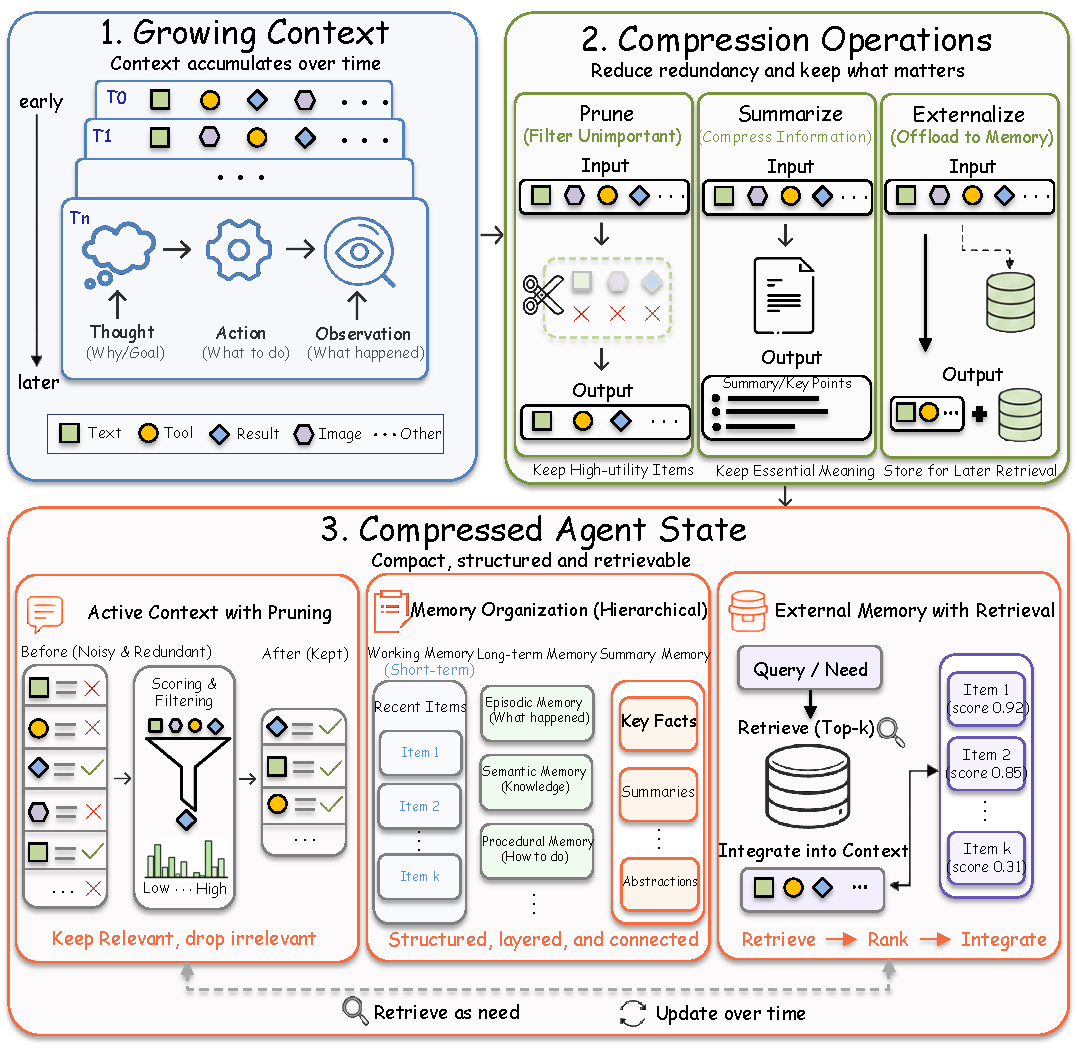
\includegraphics[width=\columnwidth]{figures/inrto.pdf}
  \vspace{-.2cm}
  \caption{Illustration of the \textit{context explosion} dilemma and the compression paradigm. Selective distillation transforms unbounded \textcolor{blue}{A-T-O sequences} into \textcolor{red}{structured representations} while preserving operational fidelity.}
  \vspace{-.4cm}
  \label{fig:agent-compression-overview}
\end{figure}



\textbf{Context compression} emerges as a highly effective pathway to mitigate this crisis, exemplified by real-world systems like \raisebox{-0.15em}{
\includegraphics[height=1em]{icons/claude-ai.pdf}}~Claude Code\footnote{\raisebox{-0.15em}{
\includegraphics[height=1em]{icons/claude-ai.pdf}}~Claude Code: https://claude.com/product/claude-code.} that proactively compact contexts upon breaching predefined trajectory thresholds. Unlike the compression of static long documents explored in prior literature~\citep{wang2026fasafrequencyawaresparseattention, li2025surveylargelanguagemodel, xiao2024efficientstreaminglanguagemodels}, the profound \textbf{structural rigidity} of A-T-O sequences in agentic trajectories renders standard text reduction inapplicable. Consequently, as conceptualized in Figure~\ref{fig:agent-compression-overview}, effective agent compression must \textbf{distill massive, noisy trajectories into compact, actionable states} while strictly \textbf{preserving causal action-observation dependencies} and structural integrity.



The prevalence of autonomous agents has catalyzed a rapid proliferation of agentic context compression techniques. These methods are scattered across different compression targets, transformation mechanisms, and control strategies, ranging from pruning and summarization to selective retrieval and representation-level interventions~\citep{lindenbauer2025complexitytrapsimpleobservation, xiao2025improving, wu2026resumunlockinglonghorizonsearch, ye2025agentfoldlonghorizonwebagents, wu2026contextweaverselectivedependencystructuredmemory, wu2026gitcontextcontrollermanage, feng2026agentocrreimaginingagenthistory, wu2026crossmodalmemorycompressionefficient}. Yet these efforts remain largely preliminary and disjointed explorations, lacking any \textbf{systematic synthesis} or \textbf{holistic perspective}. This conceptual fragmentation obscures a principled understanding of both the efficacy of underlying algorithmic designs and how specific compression choices trigger \textbf{distinct downstream agent failures}~\citep{mei2025surveycontextengineeringlarge}. Consequently, practitioners are left without a theoretical framework to navigate the complex trade-offs among \textbf{context footprint}, \textbf{structural fidelity}, and \textbf{historical recoverability}.

Prior surveys on prompt compression~\citep{jiang-etal-2023-llmlingua, li2025prompt} focus on the single-turn reduction of static inputs, whereas we study multi-turn trajectories whose relevance structure evolves over time. Work on KV cache~\citep{li2024survey, liu2025kv, mathurunderstanding} and model compression~\citep{zhu2024survey, liu2025survey, xu2023survey} addresses efficiency at the model or systems layer, while our concern is application-level context control during execution. Surveys on agent memory~\citep{tang2026llm, zhang2025survey, hu2025memory} organize methods by storage form, whereas we emphasize the intervention points, objects, and resulting forms of compressed context. Broader context engineering surveys span retrieval, memory, and orchestration at a high level~\citep{mei2025surveycontextengineeringlarge}; by contrast, we provide a focused treatment of compression as a \textbf{first-class operational capability} in agent systems.

As agents enter the era of long-horizon tasks, context compression has become a three-dimensional systems problem rather than a single-turn prompt optimization trick. Yet a systematic review of this emerging domain remains absent. To fill this gap, we introduce a unified taxonomy organized around three questions: \textbf{\textit{compression target}} (what is compressed), \textbf{\textit{compression mechanism}} (how it is transformed and retained), and \textbf{\textit{control policy}} (who decides when compression is triggered). These dimensions map directly onto the operational pipeline: targets specify \textbf{Select}, mechanisms instantiate \textbf{Compress} and \textbf{Store}, and policies govern when these stages, and when needed \textbf{Recover}, are activated. We further formalize three recurring failure modes, \fone, \ftwo, and \fthree, and use them to expose reliability trade-offs. Finally, we critique current evaluation paradigms~\citep{liu2025agentbenchevaluatingllmsagents} and argue for metrics beyond end-task success, including information density, temporal consistency, and error propagation.

The rest of the survey is organized as follows. Section~\ref{sec:2_background} introduces the background and unified pipeline, Section~\ref{sec:3_formal_view} presents a formal lens, Sections~\ref{sec:3_taxonomy} and~\ref{sec:4_failure_modes} develop the taxonomy and failure analysis, and the remaining sections discuss domain-specific trade-offs, evaluation, future directions, and conclusion.



\section{Redefining Context: From Static Prompts to Dynamic Trajectories}
\label{sec:2_background}
\subsection{What Is Unique About Agent Context}
\label{subsec:what_is_unique}

Formally, agent context is a time-indexed state $C_t$ continuously updated by interaction tuples $x_t = (a_t, t_t, o_t)$ of actions, thoughts, and observations~\citep{yao2023reactsynergizingreasoningacting}. Unlike standard long-text processing, this dynamic trajectory exhibits four fundamental properties that distinguish it from static prompts:

\noindent\textbf{Property 1: Dynamic Growth.} Context is not provided all at once but expands incrementally by absorbing new interactions $x_t$ with each agent step. Unlike static documents with fully exposed structures, agentic compression operates blindly on this continuous stream, dynamically distilling history without foreseeing future states.

\noindent\textbf{Property 2: Heterogeneous Composition.} Context comprises highly distinct structured content, including natural language plans, code snippets, JSON tool outputs, screenshots, and error logs. While natural language thoughts ($t_t$) may endure lossy abstraction, actions and observations often demand strict syntactic fidelity, mandating type-aware rather than uniform compression.

\noindent\textbf{Property 3: Multi-step Dependency.} Information compressed or discarded at a certain step may only be needed several steps later. Driven by continuous streaming, the utility of any specific tuple component $e$ manifests over future steps: $\mathcal{U}(e) = \mathbb{E}\left[ \sum_{\tau = t}^{T} \gamma^{\tau - t} \cdot u_\tau(e) \right]$. Consequently, it is inherently difficult to predict future demands during compression, as the true importance of $e$ remains unobservable at time $t$.

\noindent\textbf{Property 4: Error Propagation.} Errors or omissions introduced by compression are not discovered locally. Instead, a state distortion $\delta_t = d(C_t, \tilde{C}_t)$ propagates backward along the trajectory: $C_{t+k} = U^{(k)}(\tilde{C}_t, x_{t+1:t+k})$. These errors accumulate irreversibly and are treated as factual grounding by subsequent reasoning steps, permanently shifting the action space and derailing the agent from the optimal path.

\vspace{1ex}
\noindent\textit{\textbf{$\blacktriangleright$ Why Traditional Compression Fails $\blacktriangleleft$}} Traditional methods satisfy one-off budget constraints by optimizing for immediate relevance~\citep{jiang-etal-2023-llmlingua, jiang2024longllmlinguaacceleratingenhancingllms}. For example, KV cache compression typically evicts tokens with low current attention scores~\citep{xiao2024efficientstreaminglanguagemodels, NEURIPS2024_28ab4182}. However, under the four properties above, applying such static interventions to an evolving agentic loop triggers compounding distortions, as continuous interaction defies any static definition of information importance.


\subsection{A Unified Operational Pipeline for Agent Context Compression}
\label{subsec:unified_pipeline}

% Existing methods for agent context compression are fragmented, making it difficult to compare systems or reason about where compression intervenes in execution.
We formulate a unified four-stage pipeline that decomposes compression into an operator system over the context lifecycle:

{\setlength{\abovedisplayskip}{4pt}
\setlength{\belowdisplayskip}{4pt}
\setlength{\abovedisplayshortskip}{2pt}
\setlength{\belowdisplayshortskip}{2pt}
\vspace{-.3cm}
\begin{equation}
    C_{t+1} = \underbrace{R(q_{t+1}, \mathcal{M}_{t})}_{\text{Recover}} \oplus \underbrace{M\Big(\Phi\big(S(C_{t})\big)\Big)}_{\text{Store} \leftarrow \text{Compress} \leftarrow \text{Select}} \oplus \ x_{t+1} \label{eq:pipeline}
\end{equation}
}

% This formulation operationalizes the following four chronological stages:
\begin{itemize}[leftmargin=*, parsep=0pt, topsep=1pt, itemsep=1pt]
    \item \textbf{Select ($S$):} A critical triage phase where the system determines which subsets of the context require compression and which demand exact preservation.
    \item \textbf{Compress ($\Phi$):} Specific reductive or structural transformations, ranging from simple truncation to latent encoding, are executed on the selected subset.
    \item \textbf{Store ($M$):} The resulting compressed representations are committed either to the active working memory or offloaded to an external storage state \(\mathcal{M}_t\).
    \item \textbf{Recover ($R$):} Driven by the necessity of deferred utility, relevant compressed information is selectively retrieved and decoded from \(\mathcal{M}_t\) using the current query \(q_{t+1}\).
\end{itemize}

% This four-stage formulation decouples context management from the agent's active reasoning loop. Compression thus acts as a backend state-management subsystem concerned with information density and recoverability; the next two sections make this view explicit through a formal lens and a taxonomy.

% \subsection{Why Long-Context Windows Are Not a Panacea}
% 
% A natural objection is that long-context models should render compression unnecessary. In practice, larger windows help, but they do not remove the underlying problem.
% 
% First, longer contexts do not eliminate economic constraints. Even when a model can technically accept more tokens, inference cost, latency, and memory usage still grow with context length. In interactive agent systems, these costs remain material~\citep{hooper-etal-2025-squeezed, liu2024retrievalattentionacceleratinglongcontextllm}.
% 
% Second, more context is not equivalent to better context use. Empirical studies by \citet{liu2023lostmiddlelanguagemodels} on long-context models show that information in long prompts may be underutilized, and that simply increasing the window does not guarantee improved retrieval or reasoning. The issue is therefore not only capacity, but utilization~\citep{kim-etal-2025-really, tian-etal-2025-distance}.
% 
% Third, the central concern is information quality, not token count alone. A long but noisy trajectory can still degrade planning, dilute salient constraints, and increase brittleness. Compression is thus a mechanism for improving information density, not merely for fitting within a budget~\citep{du-etal-2025-context}.
% 
% In short, a larger context window raises the ceiling; context compression raises the floor.



\section{Compression as Sufficient State Approximation}
\label{sec:3_formal_view}
% This section reframes agent context compression as sufficient-state approximation. The point is not to introduce a new optimization algorithm, but to state the objective that existing methods only approximate: the shortest representation that still supports future action.
% \begin{figure*}[ht]
%     \centering
%     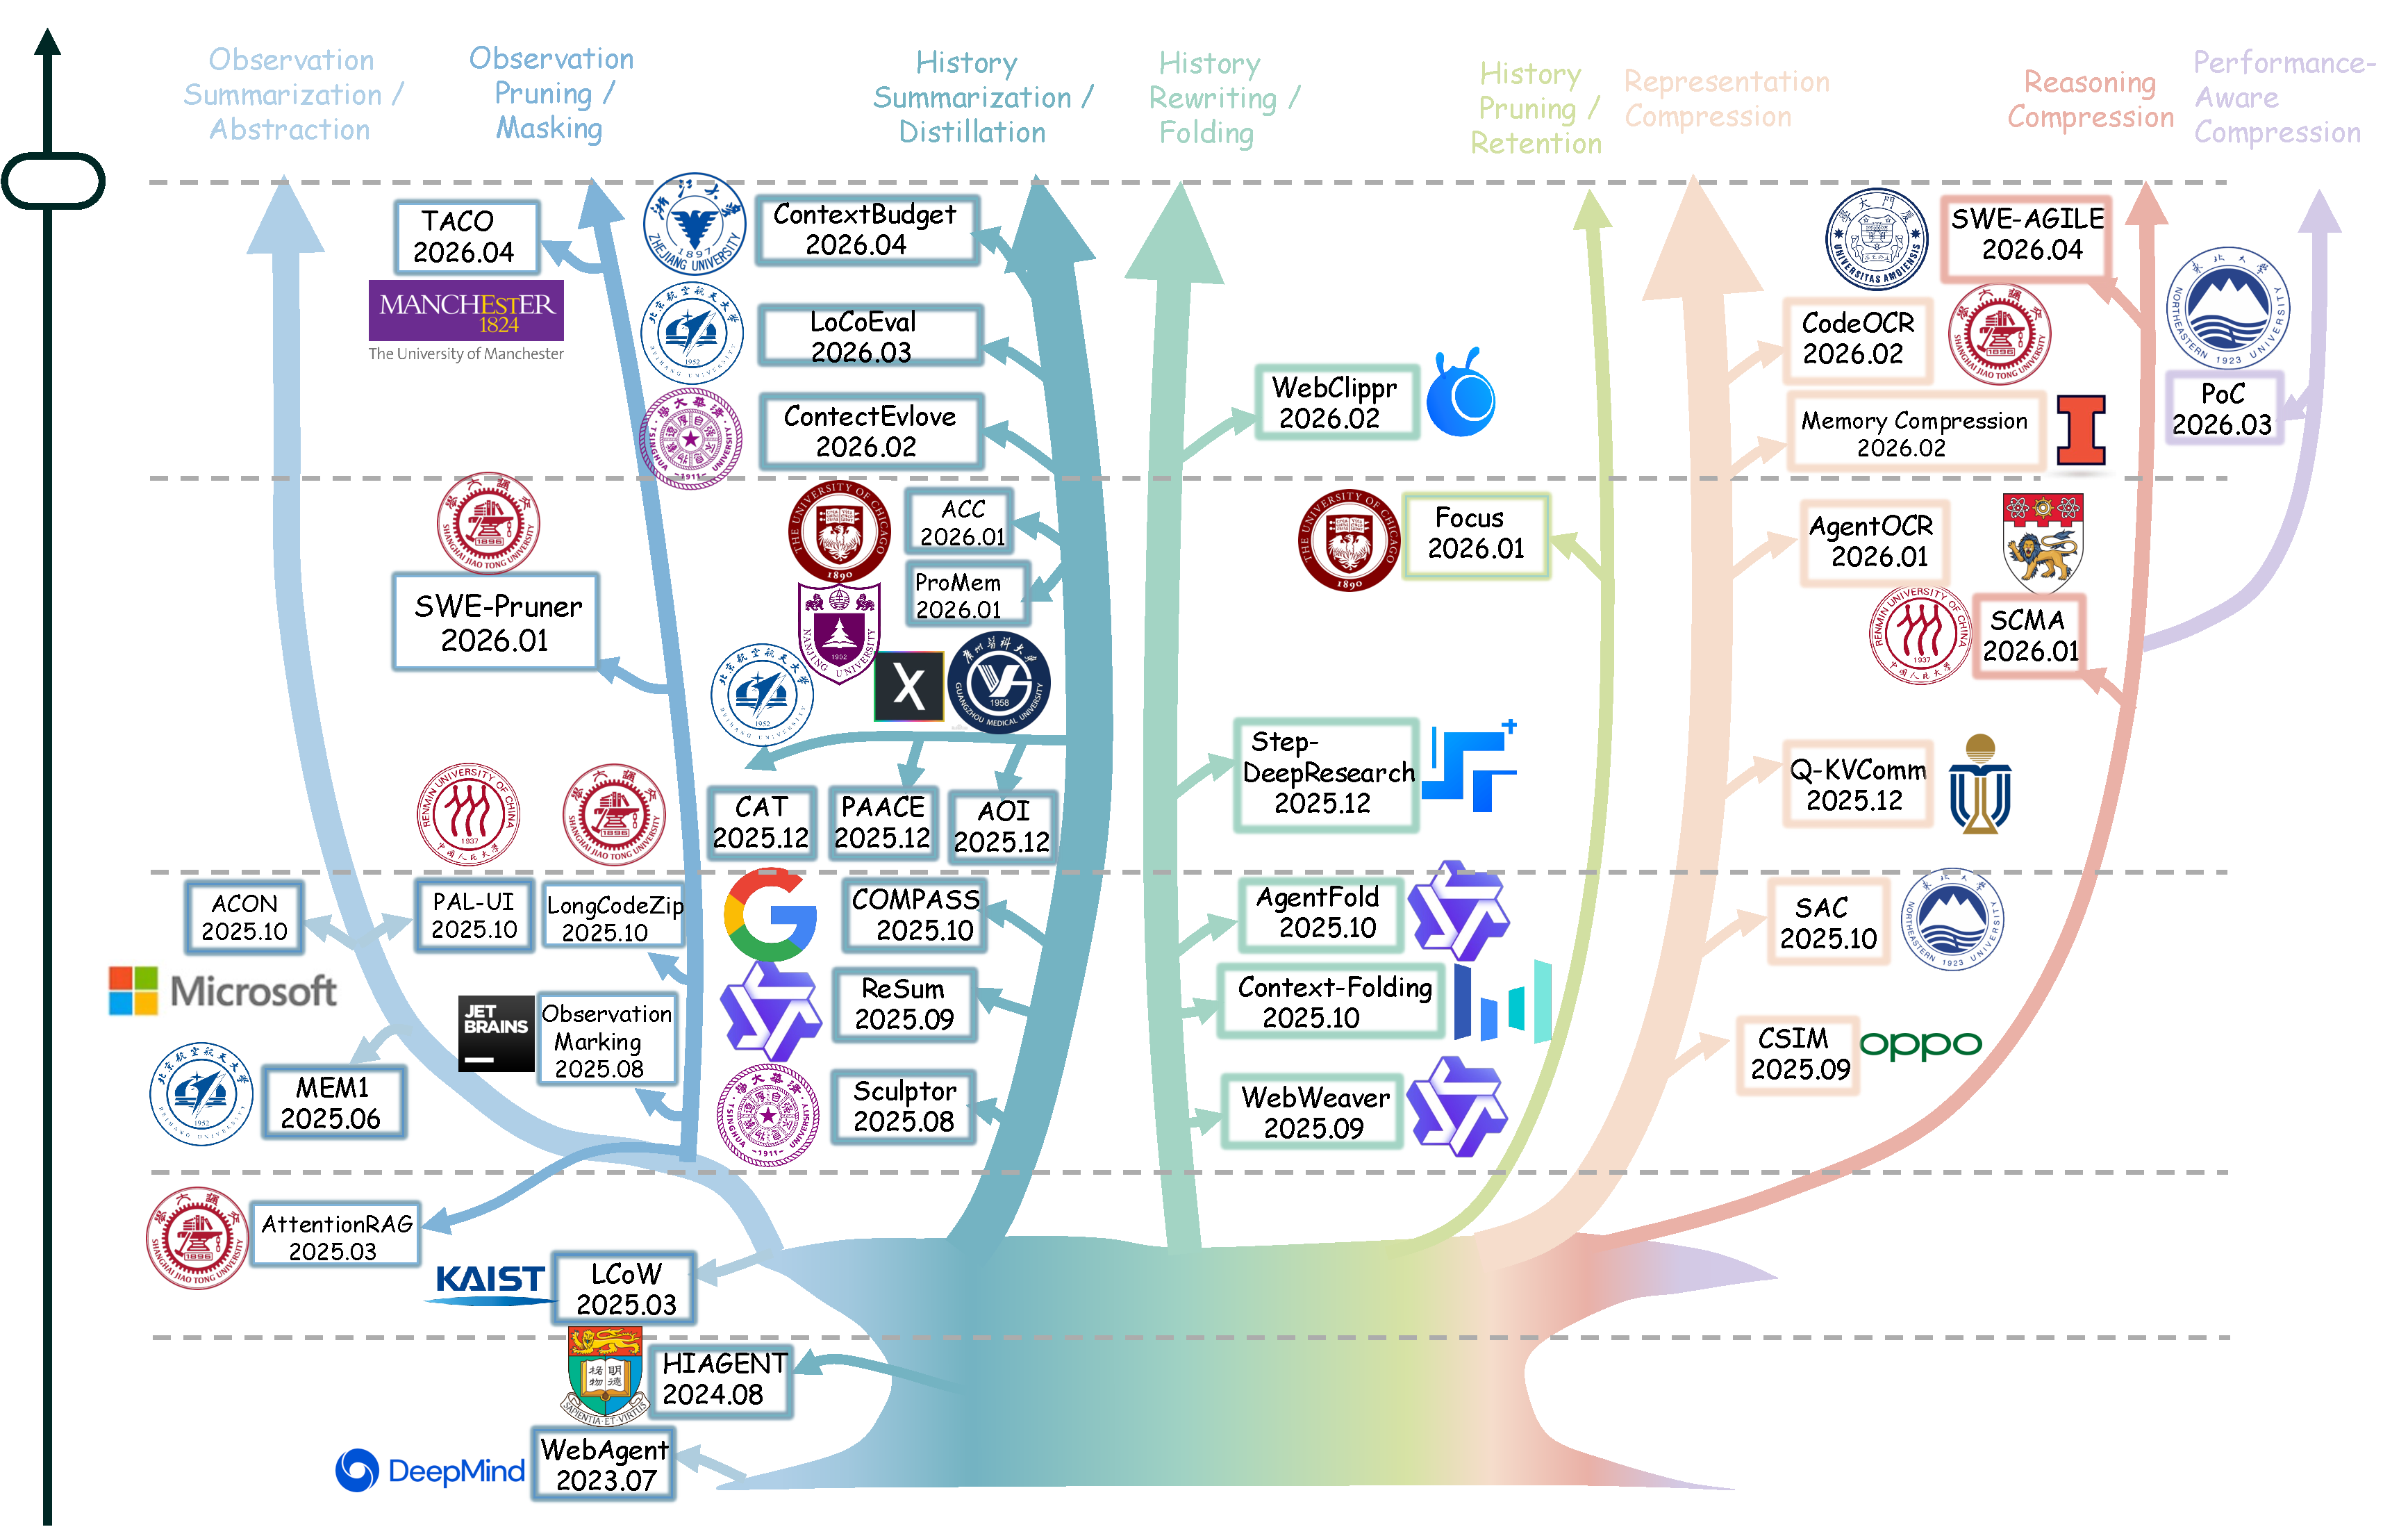
\includegraphics[width=0.74\textwidth]{figures/taxonomy.pdf}
%     \vspace{-.2cm}
%     \caption{A design-space view of agent context compression. The figure synthesizes targets, mechanisms, and control policies into a method-level landscape, grouping approaches by compression semantics while preserving chronological evolution. See Appendix~\ref{app:methodology} and \ref{ap:extended_taxonomies} for methodology, taxonomy details, and open-source resources.}
%     \label{fig:taxonomy_tree}
% \vspace{-.4cm}
% \end{figure*}

We argue that agent context compression is best understood as a sufficient-state approximation problem: the goal is to maintain the shortest representation that remains sufficient for future action.

\paragraph{Compression as State Transformation.} Let \(C_t\) denote the current context state. We treat each compression method as a transformation
{\setlength{\abovedisplayskip}{4pt}
\setlength{\belowdisplayskip}{4pt}
\setlength{\abovedisplayshortskip}{2pt}
\setlength{\belowdisplayshortskip}{2pt}
\[
O_i : \mathcal{C} \rightarrow \mathcal{C}, \qquad C_t' = O_i(C_t),
\]
}
where \(O_i\) maps \(C_t\) to a shorter, reorganized, or externally mediated representation \(C_t'\) under task-specific constraints. This abstraction is deliberately broad. It covers the operator families discussed later in the survey, including truncation, pruning, summarization, externalization, and representation-level compression.


\paragraph{Ideal Sufficient Memory.} From an algorithmic-information perspective, these operators can be viewed as practical approximations to an ideal sufficient memory. Let \(E_t\) denote the currently accessible environment state, \(A\) the agent policy or executor, \(\tau\) the task or task distribution, and \(\epsilon\) the maximum acceptable degradation in downstream performance. We define the ideal sufficient memory length as
\vspace{-.2cm}
\begin{equation}
\label{eq:ideal_sufficient_memory}
\begin{aligned}
L_{\epsilon}(C_t)
=
\min_{\tilde C_t \in \mathcal{S}_t}
&\ K(\tilde C_t \mid E_t) \\
\mathrm{s.t.}\quad
&\Delta_{\tau}(A; C_t,\tilde C_t,E_t) \leq \epsilon ,
\end{aligned}
\end{equation}
\vspace{-.1cm}
where \(\mathcal{S}_t = \mathcal{S}(C_t,E_t)\) denotes the admissible space of compressed states derived from \(C_t\) under environment \(E_t\). Here \(K(\tilde C_t \mid E_t)\) is standard conditional Kolmogorov complexity, and \(\Delta_{\tau}(A; C_t,\tilde C_t,E_t)\) measures the loss in future task performance induced by replacing \(C_t\) with \(\tilde C_t\). The quantity \(L_{\epsilon}\) is not meant as a computable training objective; rather, it serves as a stylized lower bound. A compressed state is useful only insofar as it remains compact, task-sufficient, and recoverable for future decisions.

\paragraph{From Approximation to Failure.} This objective turns the next two sections into one question: how does a method approximate a sufficient future state, and where can that approximation fail? Truncation bets that dropped spans have no future value. Pruning preserves an exact sufficient subset. Summarization replaces evidence with an executable abstraction. Externalization keeps part of the sufficient state off-context and shifts the bottleneck to recovery. Representation-level compression pushes sufficiency into latent space and sacrifices transparency. Under this view, the taxonomy compares approximation strategies, while the failure modes identify where sufficiency or recoverability is lost.




\section{A Taxonomy of Agent Compression}
\label{sec:3_taxonomy}
\subsection{From Pipeline to Design Space}
\label{subsec:design_space}

\newcommand{\compacteq}[1]{%
{\setlength{\abovedisplayskip}{3pt}%
\setlength{\belowdisplayskip}{3pt}%
\setlength{\abovedisplayshortskip}{1pt}%
\setlength{\belowdisplayshortskip}{1pt}%
\[
#1
\]}}

% \begin{figure*}[ht]
%     \centering
%     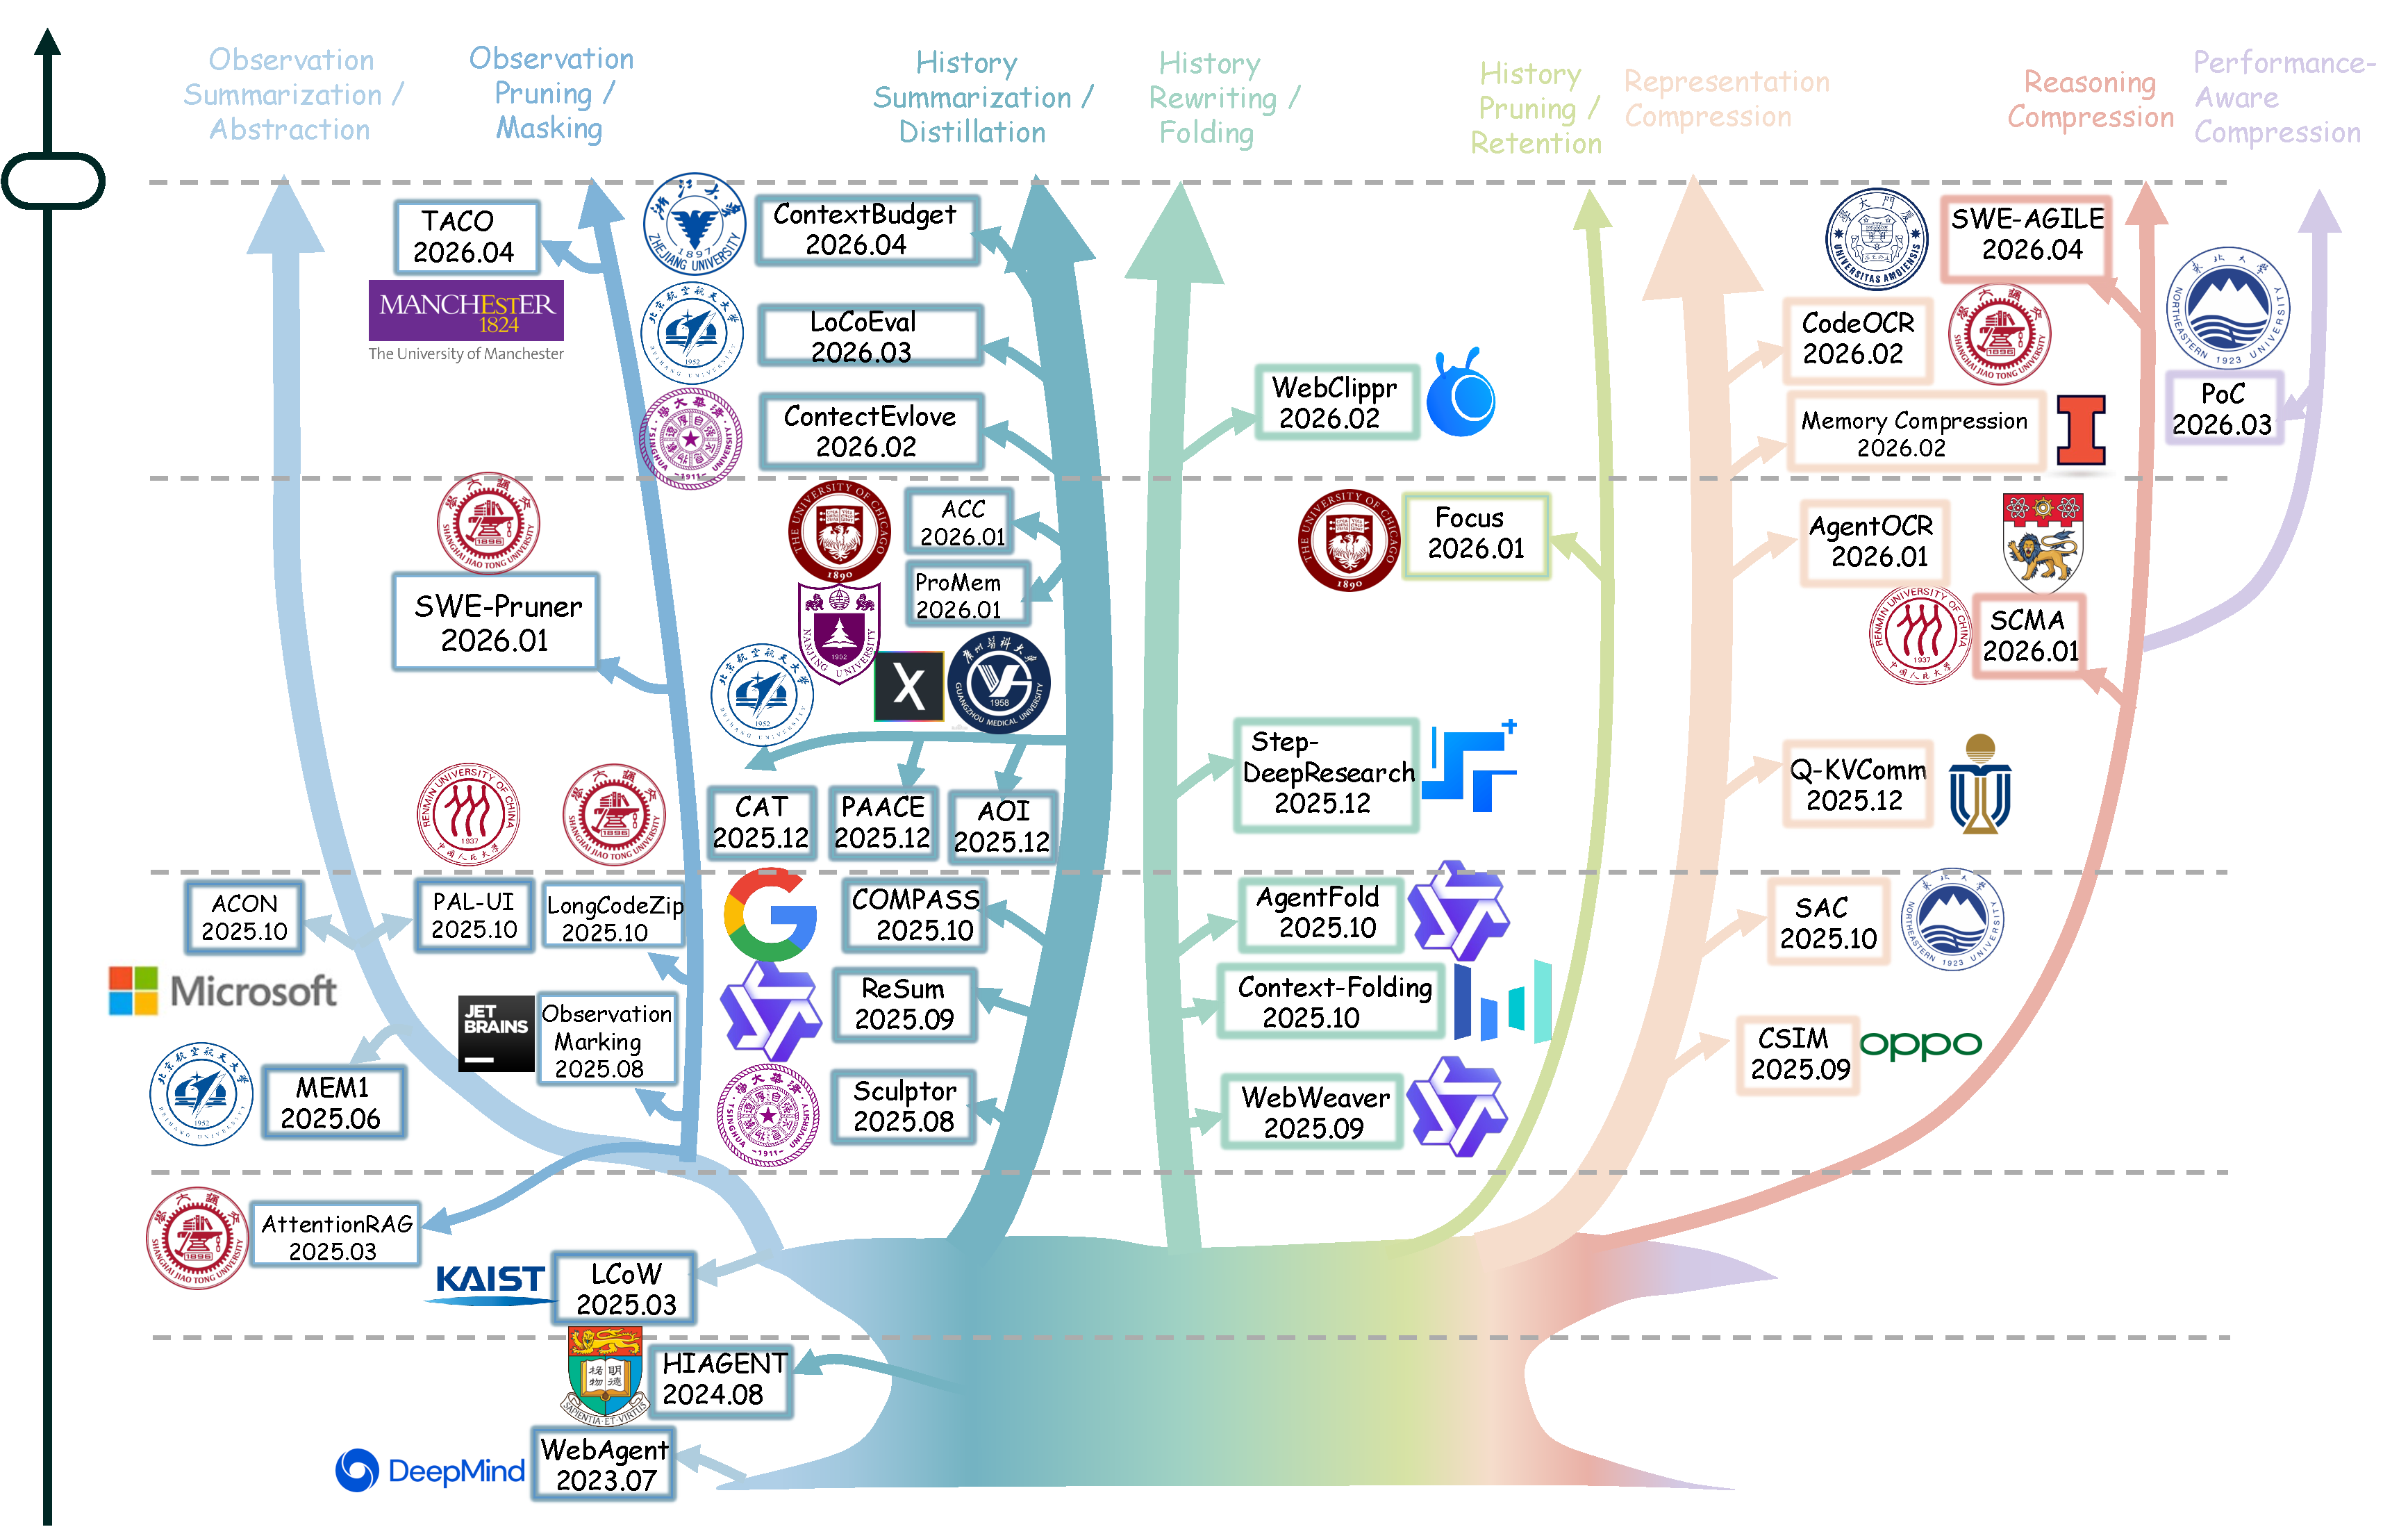
\includegraphics[width=0.74\textwidth]{figures/taxonomy.pdf}
%     \vspace{-.2cm}
%     \caption{A design-space view of agent context compression. The figure synthesizes targets, mechanisms, and control policies into a method-level landscape, grouping approaches by compression semantics while preserving chronological evolution.}
%     \label{fig:taxonomy_tree}
% \end{figure*}


The unified pipeline in \S~\ref{subsec:unified_pipeline} can be read as a comparative design space for agent compression. We organize the literature along three axes: \textit{what} is selected for compression, \textit{how} it is transformed, and \textit{who} decides when compression occurs. These axes map naturally onto the pipeline: targets define the input to \textbf{Select} ($S$), mechanisms implement \textbf{Compress} ($\Phi$) and \textbf{Store} ($M$), and control policies govern when these stages, and when necessary \textbf{Recover} ($R$), are invoked.
\vspace{0.8em}

\begin{table*}[t]
\centering
\small
\begin{tabular}{@{}p{2.4cm}p{2.6cm}p{1.5cm}p{1.5cm}p{1.8cm}p{3.5cm}@{}}
\toprule
\textbf{\raisebox{-0.15em}{
\includegraphics[height=1em]{icons/target.pdf}}~Target} & \textbf{\raisebox{-0.15em}{
\includegraphics[height=1em]{icons/pyramid.pdf}}~Granularity} & \textbf{Information Density} & \textbf{Causal Coupling} & \textbf{Recoverability} & \textbf{\raisebox{-0.15em}{
\includegraphics[height=1em]{icons/failure.pdf}}~Typical Failure Symptom} \\
\midrule
\textbf{Observation} & Token / Segment & Very Low & Weak & Low & Structural Distortion \\
\textbf{Trajectory} & Episode & Low & Moderate & Moderate & Planning Drift \\
\textbf{Plan \& Reasoning} & State & High & Very Strong & Very Low & Metacognitive Error \\
\textbf{Memory State} & State & High & Strong & Very Low & Retrieval Blindness \\
\textbf{Representation} & Token / Latent & Very High & None & None & Semantic Collapse \\
\bottomrule
\end{tabular}
% \vspace{-.2cm}
\caption{A comparative anatomy of compression targets. Each target is characterized by its granularity, information density, causal coupling, and recoverability, which collectively shape its compressibility and its failure symptom.}
\label{tab:target_comparison}
\vspace{-.2in}
\end{table*}

\subsection{Compression Targets (\textit{What})}
\label{subsec:compressin_target}

We begin with the objects processed by the \textbf{Select} ($S$) operator. Table~\ref{tab:target_comparison} summarizes these targets in terms of granularity, information density, causal coupling, and recoverability. Together, these properties determine both compressibility and likely failure symptoms.

\subsubsection{Observation Compression}
Observation compression targets raw inputs, such as tool outputs, HTML DOMs, logs, or screenshots. These inputs are high-volume and redundant, but a single omitted selector, trace line, or visual cue may determine the next action. Methods such as The Complexity Trap~\citep{lindenbauer2025complexitytrapsimpleobservation} therefore treat it as a low-cost front-end intervention, typically via masking or shallow filtering.

\subsubsection{Trajectory Compression}
Trajectory compression focuses on accumulated multi-step histories, including failed attempts, redundant tool calls, and repetitive loops. Its main difficulty is deferred utility: information that appears irrelevant at step $t$ may become indispensable later. As a result, trajectory compression is especially vulnerable to \ftwo \quad and delayed downstream inconsistency. Representative approaches include controller-mediated reduction in AgentDiet~\citep{xiao2025improving}, periodic summarization in ReSum~\citep{wu2026resumunlockinglonghorizonsearch}, and proactive folding in AgentFold~\citep{ye2025agentfoldlonghorizonwebagents}.

\subsubsection{Plan and Reasoning Compression}
Plan and reasoning compression targets internal artifacts, including subgoals, deliberative traces, self-reflections, and task decompositions. These representations are compact but brittle: dropping a seemingly minor premise can invalidate an entire downstream plan. This target is therefore  sensitive to \fone, because the system must correctly judge which reasoning artifacts remain decision-critical. Representative methods include feedback-driven summarization in ACON~\citep{kang2025aconoptimizingcontextcompression} and agent-initiated memory management in Focus~\citep{verma2026activecontextcompressionautonomous}.


\subsubsection{Memory State Compression}
Memory state compression maps an unbounded interaction stream into a fixed-capacity representation that survives beyond the immediate context window. It most explicitly realizes the \textbf{Store} ($M$) stage, so its main bottleneck is accessibility rather than faithfulness. Once information is offloaded, the system must still recognize when that memory matters and reconstruct it at use time. Consequently, memory-state compression is most directly exposed to \fthree. Learned memory policies such as MEM1~\citep{zhou2025mem1learningsynergizememory} address this challenge by coupling state formation with future retrieval utility.

\subsubsection{Representation-Level Compression}
Representation-level compression operates below the natural-language interface, targeting KV caches, multimodal token embeddings, or other latent states. It often delivers the strongest efficiency gains, but with minimal recoverability and weak inspectability. These methods therefore shift the problem from semantic editing to opaque state management. Representative examples include AgentOCR~\citep{feng2026agentocrreimaginingagenthistory}, Q-KVComm~\citep{kriuk2025qkvcommefficientmultiagentcommunication}, and SAC~\citep{liu2026autoencodingfreecontextcompressionllms}.


\subsection{Compression Mechanisms (\textit{How})}
\label{subsec:compression_mechanism}

% Having identified the targets, we now turn to the transformations themselves. Mechanisms differ in the relation they preserve between the compressed artifact and the source context: some delete spans outright, some rewrite them semantically, some retain only an exact subset, and others offload information into an explicitly recoverable store. This distinction is central because methods with similar compression ratios can differ sharply in faithfulness, inspectability, and downstream recoverability.
Having identified the targets, we now turn to the transformations themselves. What most distinguishes compression mechanisms is how they relate the compressed result to the original context. Some remove content, some paraphrase it, some retain an exact subset, and others store information so that it can be recovered later. This distinction is crucial because methods with similar compression ratios may differ sharply in \emph{faithfulness}, \emph{inspectability}, and \emph{downstream recoverability}.

\subsubsection{Masking and Truncation} 
These operators keep a prefix or suffix of the context, or selectively mask designated spans:
\compacteq{O_{\mathrm{trunc}}(\mathcal{C}) = \mathcal{C}[:k],\; O_{\mathrm{mask}}(\mathcal{C}) = \mathrm{mask}(\mathcal{C}, S).}
These operators, which directly modify the support of \(C\) through span removal or placeholder substitution, are universal, low-overhead, and easy to deploy. That same directness also defines their limitation: once content is removed, recoverability is lost unless another subsystem stores it elsewhere. Such operators are therefore best suited to settings in which marginal utility decays rapidly with recency or position, as in sliding-window baselines or hard budget enforcement~\citep{wang2025mcpbenchbenchmarkingtoolusingllm}.

\subsubsection{Summarization and Abstraction} 
These operators rewrite a long context into a shorter semantic representation:
\compacteq{O_{\mathrm{sum}}(\mathcal{C}) = \hat{C},\; |\hat{C}| \ll |\mathcal{C}|.}
Unlike truncation, summarization preserves utility by semantic rewriting rather than direct deletion. This often yields substantially higher information density and better long-horizon compactness, which explains its popularity in research and search agents. The trade-off is that faithfulness becomes model-dependent: once context is rewritten, omissions, over-generalizations, and spurious inferences may be introduced, making summarization a primary locus of \ftwo. Representative systems include LCoW~\citep{lee2025learningcontextualizewebpages}, COMPASS~\citep{wan2025compassenhancingagentlonghorizon}, and ReSum~\citep{wu2026resumunlockinglonghorizonsearch}.


% \subsubsection{Masking and Truncation} 
% These operators keep a prefix or suffix of the context, or selectively mask designated spans:
% \compacteq{O_{\mathrm{trunc}}(\mathcal{C}) = \mathcal{C}[:k],\; O_{\mathrm{mask}}(\mathcal{C}) = \mathrm{mask}(\mathcal{C}, S).}
% They directly modify the support of \(C\) through span removal or placeholder substitution. Their appeal lies in universality, low overhead, and ease of deployment. Their limitation is equally direct: once content is removed, recoverability is lost unless another subsystem stores it elsewhere. These operators are therefore best suited to settings in which marginal utility decays rapidly with recency or position, as in sliding-window baselines or hard budget enforcement~\citep{wang2025mcpbenchbenchmarkingtoolusingllm}.

% \subsubsection{Summarization and Abstraction} 
% These operators rewrite a long context into a shorter semantic representation:
% \compacteq{O_{\mathrm{sum}}(\mathcal{C}) = \hat{C},\; |\hat{C}| \ll |\mathcal{C}|.}
% Unlike truncation, they preserve utility by semantic rewriting rather than direct deletion. This often yields substantially higher information density and better long-horizon compactness, which explains their popularity in research and search agents. The trade-off is that faithfulness becomes model-dependent: once context is rewritten, omissions, over-generalizations, and spurious inferences may be introduced, making summarization a primary locus of \ftwo. Representative systems include LCoW~\citep{lee2025learningcontextualizewebpages}, COMPASS~\citep{wan2025compassenhancingagentlonghorizon}, and ReSum~\citep{wu2026resumunlockinglonghorizonsearch}.

\subsubsection{Pruning and Reduction} 
Pruning removes content selectively while preserving the remaining structure exactly:
\compacteq{O_{\mathrm{prune}}(\mathcal{C}) = \mathcal{C} \setminus R,}
where \(R\) is a subset selected by a relevance, dependency, or structural criterion. Unlike summarization, pruning leaves retained evidence untouched. It is therefore especially valuable when syntactic form, pointer alignment, or execution traces must remain exact, as in coding and GUI settings. In exchange, pruning typically compresses less aggressively than summarization unless the context contains substantial redundancy. Representative examples include SWE-Pruner~\citep{wang2026sweprunerselfadaptivecontextpruning} and WebClipper~\citep{wang2026webclipperefficientevolutionweb}.

\subsubsection{Externalization and Retrieval} 
This mechanism splits context into a working state and an external store:
\compacteq{O_{\mathrm{ext}}(\mathcal{C}) = (C', M),\; O_{\mathrm{ret}}(\mathcal{C}, M) = \mathcal{C} \oplus r(M).}
It is the clearest realization of \textbf{Store} ($M$) and \textbf{Recover} ($R$) in the pipeline. By turning part of compression into retrieval, it permits aggressive footprint reduction so long as critical information can later be reconstructed on demand. It is therefore the only mechanism that combines high compression with principled recoverability. Its main risk shifts toward \fthree: not corruption, but missing, mistimed, or incorrect re-access. Systems such as Step-DeepResearch~\citep{hu2025stepdeepresearchtechnicalreport}, CAT~\citep{liu2025contexttoolcontextmanagement}, and WebWeaver~\citep{li2025webweaverstructuringwebscaleevidence} rely heavily on this paradigm.

% \subsubsection{Externalization and Retrieval} 
% This mechanism splits context into a working state and an external store:
% \compacteq{O_{\mathrm{ext}}(\mathcal{C}) = (C', M),\; O_{\mathrm{ret}}(\mathcal{C}, M) = \mathcal{C} \oplus r(M).}
% It is the clearest realization of \textbf{Store} ($M$) and \textbf{Recover} ($R$) in the pipeline. Conceptually, it converts part of the compression problem into a retrieval problem: instead of forcing all useful information to remain in the active context, it permits aggressive footprint reduction so long as critical information can later be reconstructed on demand. This makes it the only mechanism that simultaneously supports high compression and principled recoverability. Its failure mode is correspondingly shifted toward \fthree, because the main risk is no longer only information corruption but missing, mistimed, or incorrect re-access. Systems such as Step-DeepResearch~\citep{hu2025stepdeepresearchtechnicalreport}, CAT~\citep{liu2025contexttoolcontextmanagement}, and WebWeaver~\citep{li2025webweaverstructuringwebscaleevidence} rely heavily on this paradigm.
% \begin{figure*}[t]
%     \centering
%     \captionbox{A temporal taxonomy of context compression failures. Failures are classified by the earliest point at which they occur in the compression pipeline.\label{fig:failure_modes_taxonomy}}[0.48\textwidth]{%
%     \makebox[\linewidth][l]{%
%         \raisebox{-0.3mm}[0pt][0pt]{%
%             \scalebox{1}[1.1]{%
%                 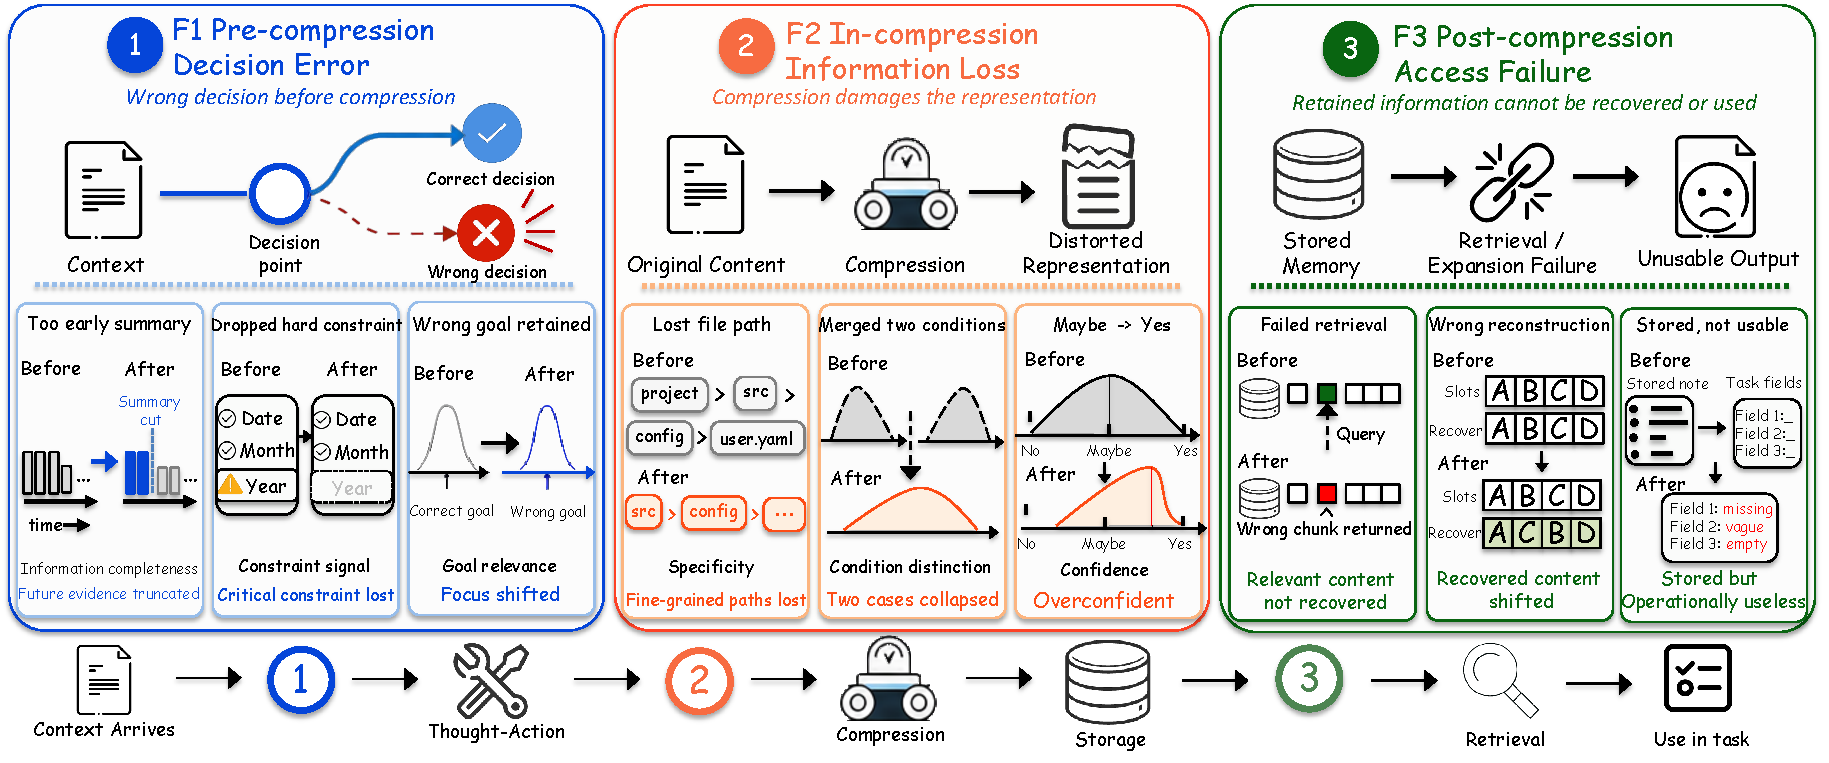
\includegraphics[width=\linewidth]{figures/section5.pdf}%
%             }%
%         }%
%     }%
%     \vspace{-.2cm}
% }
%     \hfill
%     \captionbox{Domain-specific context compression regimes, contrasting setup, workflow, interaction loop, dominant risks, and strategy choices.\label{fig:domain_specific_regimes}}[0.49\textwidth]{%
%         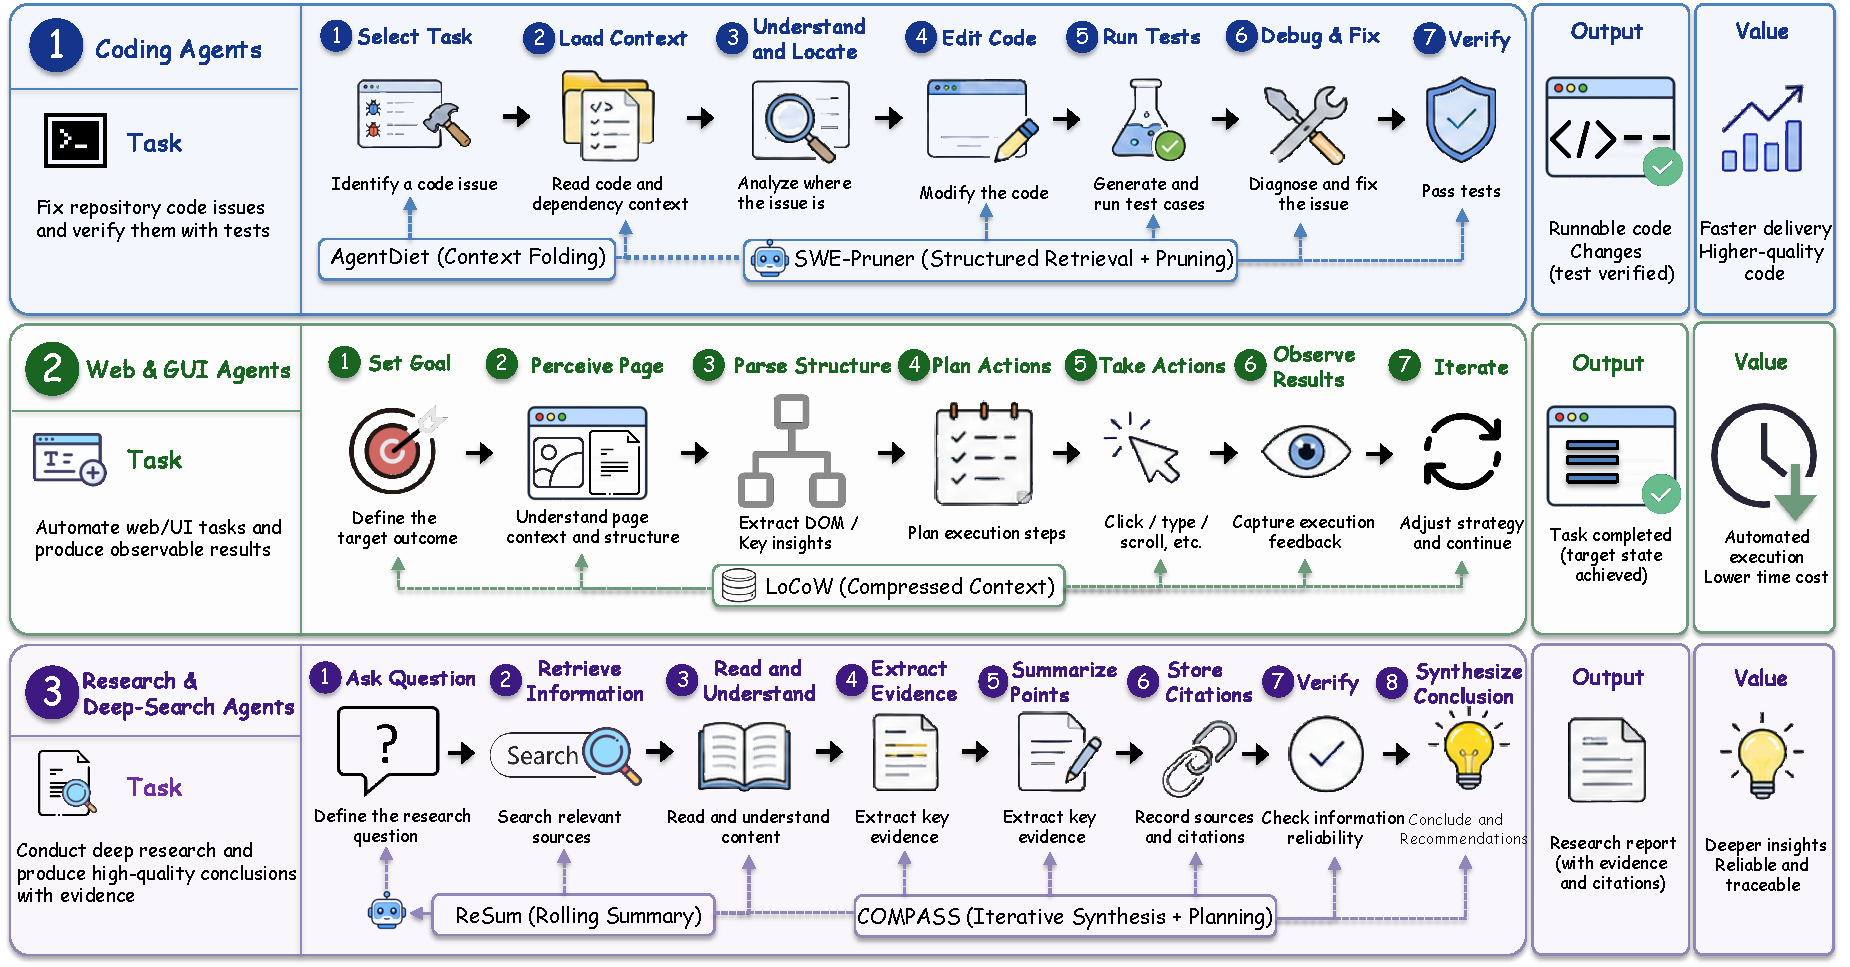
\includegraphics[width=.85\linewidth]{figures/section6.pdf}
%         \vspace{-.2cm}
%     }
% \vspace{-.3cm}
% \end{figure*}

\subsubsection{Representation Compression} 
Operating on latent structures, \(O_{\mathrm{repr}}(\mathcal{C}) = \tilde{C}\) compresses history without explicit textual rewriting. These methods optimize efficiency most directly, but they do so by moving compression beneath the symbolic interface available to the agent and the researcher. As a result, they offer limited interpretability, weak controllability, and little explicit support for exact recovery. Methods such as DebateOCR~\citep{wu2026crossmodalmemorycompressionefficient} illustrate this trade-off.


\subsection{Control Policies and Intervention Timing (\textit{Who} and \textit{When})}
\label{subsec:compression_policy}

Control policy, not compression mechanism, determines when intervention occurs. The same operator may be triggered reactively at a budget threshold, periodically by an external controller, or proactively by the agent itself. We therefore separate operator family from control policy: policy specifies when \textbf{Select}, \textbf{Compress}, and, where applicable, \textbf{Recover} are invoked, who makes that decision, and which signals are sufficient to trigger action.


\subsubsection{System-Controlled Policies} 
System-controlled policies apply fixed rules to trigger compression:
\compacteq{\pi_{\mathrm{sys}} : \mathcal{C} \mapsto (i, \theta).}
Depending only on observable signals such as length, position, or step count, they are predictable, cheap, and easy to benchmark. Their weakness is semantic blindness: they intervene because a budget is reached, not because task utility has changed. Such policies therefore dominate early and production-constrained systems, including predefined schedules in AgentDiet~\citep{xiao2025improving} and threshold-based compaction regimes.

\subsubsection{External Controller Policies} 
External-controller policies delegate the decision to a separate module:
\compacteq{\pi_{\mathrm{ext}} : \mathcal{C} \rightarrow (i, \theta).}
The controller may be a smaller model, a planner, or a retrieval manager that observes the evolving context and selects a compression action for the main agent. This decoupling improves modularity and sometimes yields more stable control, because compression can be optimized independently of task execution. The cost is additional latency, token overhead, and a new interface on which information can be lost. Examples include PAL-UI~\citep{liu2025paluiplanningactivelookback} and AOI~\citep{bai2026aoicontextawaremultiagentoperations}.

\subsubsection{Agent-Controlled Policies} 
Agent-controlled policies make compression part of the agent's own action space:
\compacteq{\pi_{\mathrm{agent}}(C_t, s_t) \rightarrow (i, \theta),}
where \(s_t\) denotes the agent's internal state. This policy class is the most semantically aware, because the same system that reasons about the task also decides which context should be compressed, preserved, or revisited. It is therefore well suited to proactive memory management and self-reflective intervention, as in CAT~\citep{liu2025contexttoolcontextmanagement}, Focus~\citep{verma2026activecontextcompressionautonomous}, and ContextBudget~\citep{wu2026contextbudgetbudgetawarecontextmanagement}. Its weakness is precisely the agent's own fallibility: errors in self-assessment readily manifest as \fone.

\subsubsection{Learned Compression Policies} 
Learned policies optimize compression behavior from data:
\compacteq{\pi_{\mathrm{learn}} = \arg\max_{\pi} \mathbb{E}_{\tau \sim \pi} \left[ R_{\mathrm{task}}(\tau) - \lambda \, \mathrm{Cost}(\tau) \right].}
Whether trained by supervised fine-tuning or reinforcement learning, they seek to align compression decisions with downstream task return rather than handcrafted heuristics. This makes them the most expressive policy class and, in principle, the closest approximation to the ideal sufficient-memory objective in Section~\ref{sec:3_formal_view}. In practice, however, they are also the most resource-intensive and the most sensitive to reward misspecification. Representative examples include ACON~\citep{kang2025aconoptimizingcontextcompression}, MEM1~\citep{zhou2025mem1learningsynergizememory}, and related policy-learning approaches.



\section{Failure Modes}
\label{sec:4_failure_modes}
We organize context compression failures by the earliest stage at which they arise: {\fone}, {\ftwo}, and {\fthree}, as shown in Figure~\ref{fig:failure_modes_taxonomy}.

% \begin{figure*}[t]
%     \centering
%     \captionbox{A temporal taxonomy of context compression failures. Failures are classified by the earliest point at which they occur in the compression pipeline.\label{fig:failure_modes_taxonomy}}[0.48\textwidth]{%
%     \makebox[\linewidth][l]{%
%         \raisebox{-0.3mm}[0pt][0pt]{%
%             \scalebox{1}[1.1]{%
%                 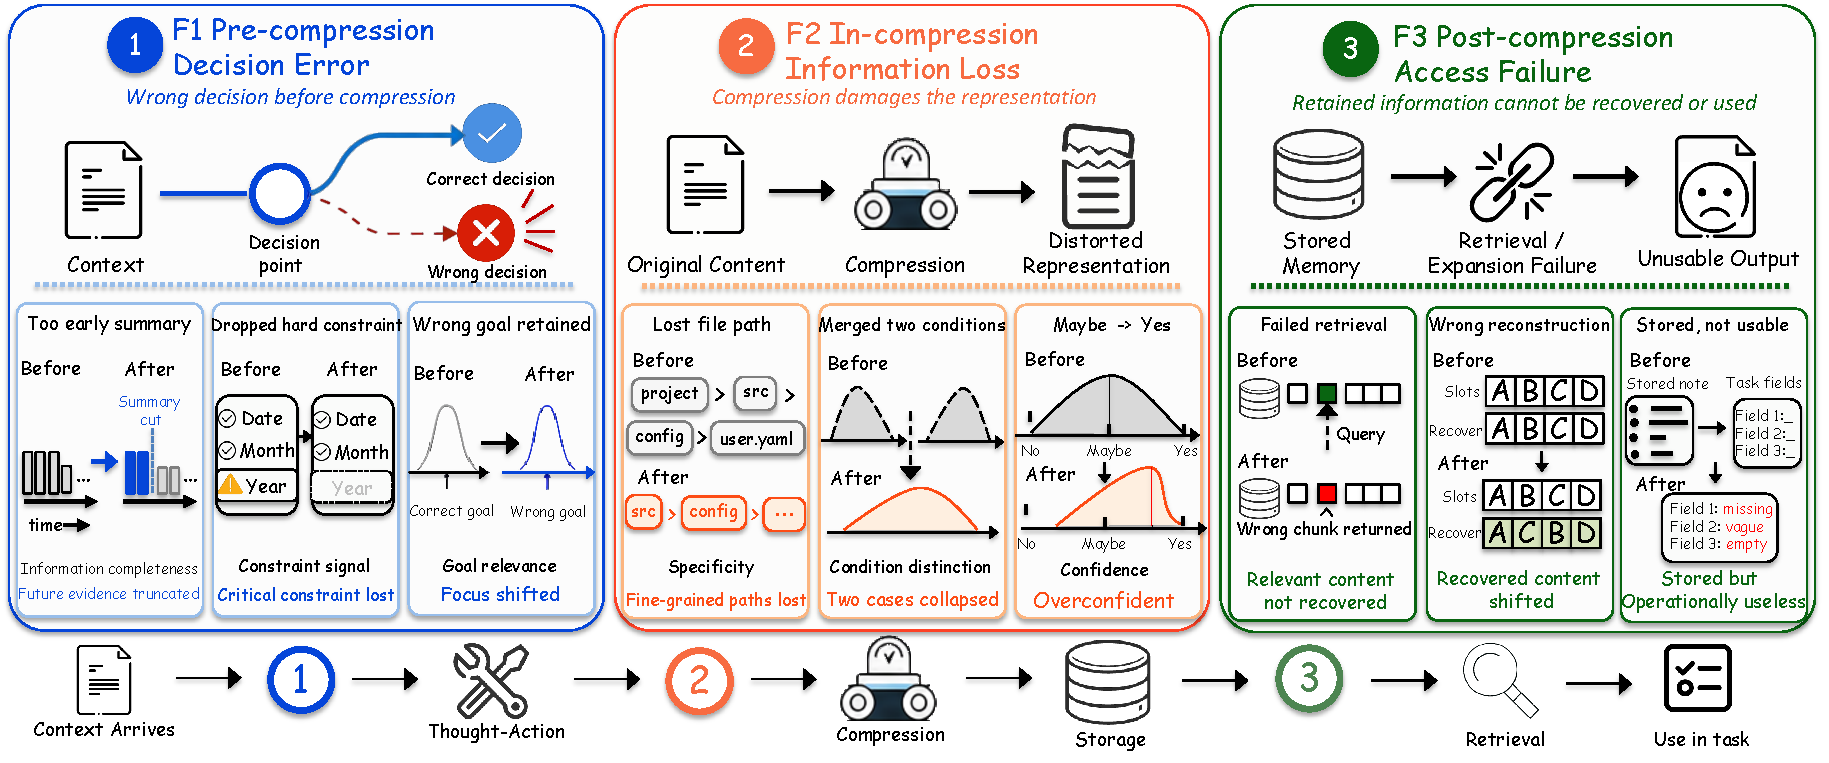
\includegraphics[width=\linewidth]{figures/section5.pdf}%
%             }%
%         }%
%     }%
%     \vspace{-.2cm}
% }
%     \hfill
%     \captionbox{Domain-specific context compression regimes, contrasting setup, workflow, interaction loop, dominant risks, and strategy choices.\label{fig:domain_specific_regimes}}[0.49\textwidth]{%
%         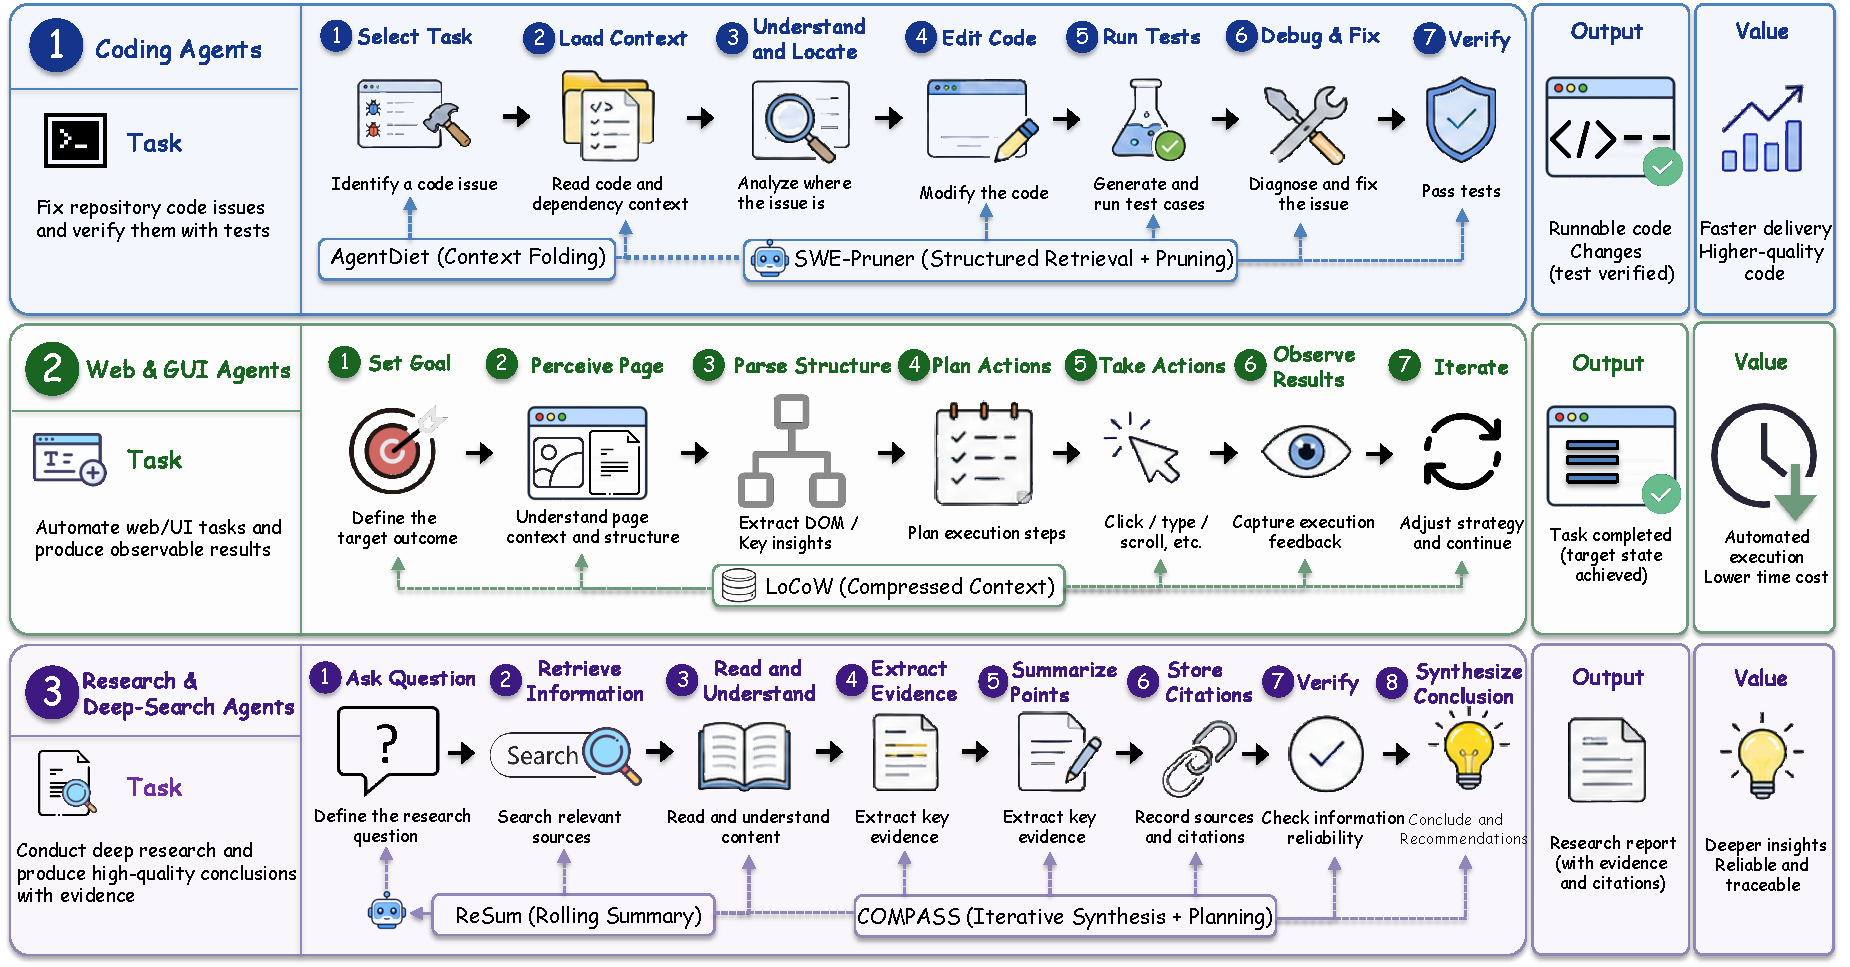
\includegraphics[width=.85\linewidth]{figures/section6.pdf}
%         \vspace{-.2cm}
%     }
% \vspace{-.2cm}
% \end{figure*}





% \begin{figure*}[t]
%     \centering
%     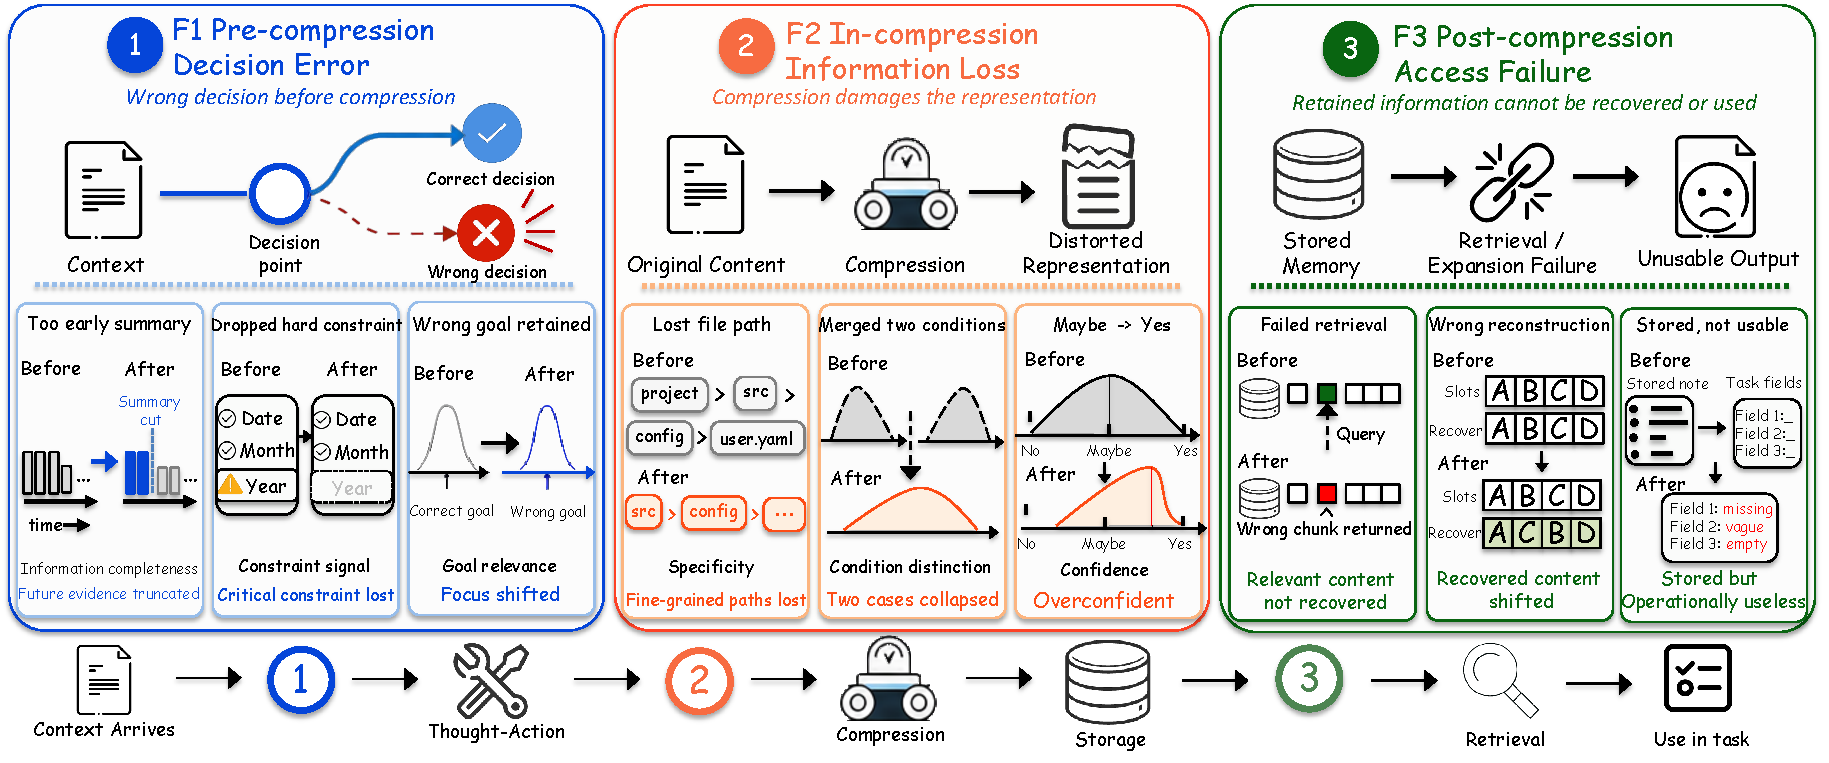
\includegraphics[width=0.5\textwidth]{figures/section5.pdf}
%     \vspace{-.2cm}
%     \caption{A temporal taxonomy of context compression failures. Failures are classified by the earliest point at which they occur in the compression pipeline: {\fone}, {\ftwo}, and {\fthree}.}
%     \label{fig:failure_modes_taxonomy}
% \end{figure*}

% \begin{figure*}[ht]
%     \centering
%     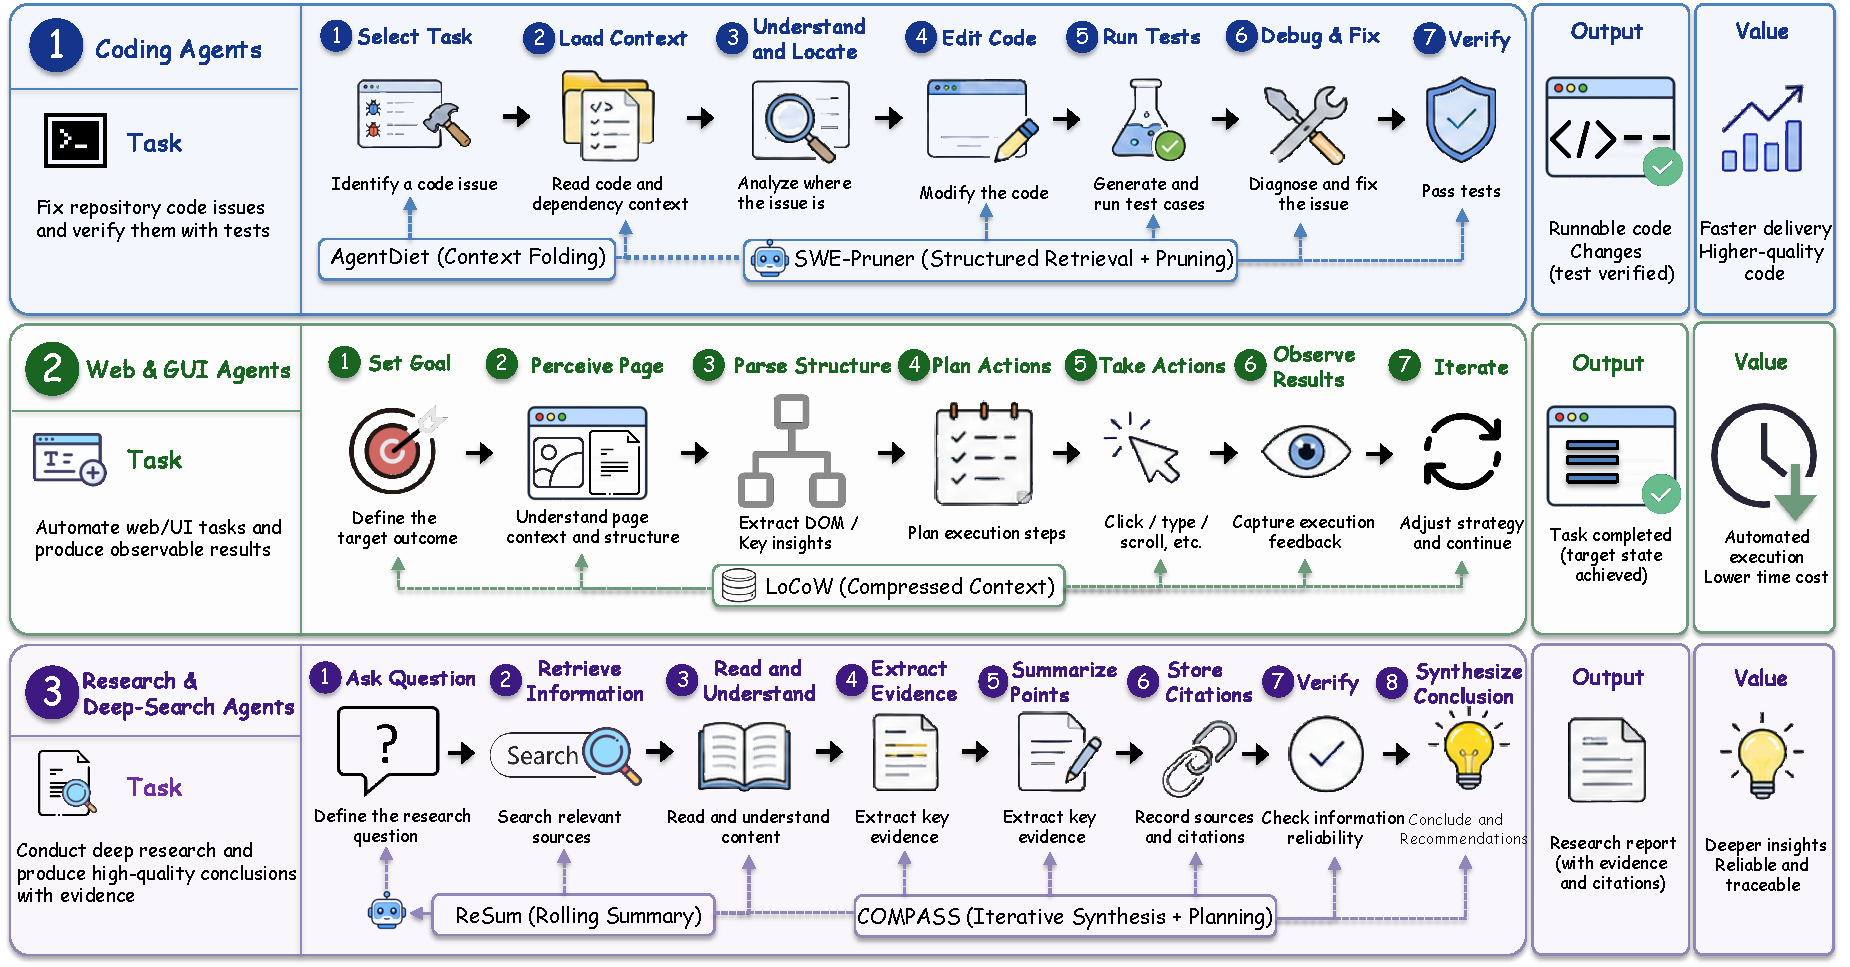
\includegraphics[width=0.5\textwidth]{figures/section6.pdf}
%     \vspace{-.2cm}
%     \caption{Domain-specific context compression regimes for coding, web/GUI, and research agents. The figure contrasts each domain's setup, workflow, interaction loop, dominant risks, and contextualized strategy choices.}
%     \label{fig:domain_specific_regimes}
% \end{figure*}

\begin{table*}[ht]
\centering
\footnotesize
\setlength{\tabcolsep}{4pt}
\setlength{\aboverulesep}{0.2ex}
\setlength{\belowrulesep}{0.2ex}
\renewcommand{\arraystretch}{0.98}
\begin{tabularx}{\textwidth}{@{}>{\raggedright\arraybackslash}p{2.2cm} >{\raggedright\arraybackslash}X >{\raggedright\arraybackslash}X >{\raggedright\arraybackslash}X >{\raggedright\arraybackslash}X@{}}
\toprule
\textbf{System} & \textbf{Select ($S$)} & \textbf{Compress ($\Phi$)} & \textbf{Store ($M$)} & \textbf{Recover ($R$)} \\
\midrule
\textbf{Claude Code} & Reactive, threshold-based selection. & Auto-compaction of prior interaction history. & Compacted state retained in active context. & Implicit recovery via continued execution. \\
\midrule
\textbf{Cursor} & Retrieval-first selection of files, code blocks, and rules. & Relevance filtering and contextual assembly. & Repository index, project rules, and workspace context. & Re-injection of retrieved files, rules, and evidence. \\
\midrule
\textbf{OpenAI Codex} & Task-grounded selection over files, instructions, and threads. & Session continuation and workspace grounding. & Task threads, instruction files, and repository state. & Recovery through continued threads and file re-access. \\
\bottomrule
\end{tabularx}
\vspace{-.2cm}
\caption{Pipeline-level comparison of recent production-grade coding agents, organized by the stages in Section~\ref{subsec:unified_pipeline}.}
\label{tab:coding_agents_pipeline}
\vspace{-.4cm}
\end{table*}

\noindent\textbf{\fone} refers to failures that arise before compression itself, when the system chooses the wrong moment, target, or granularity of compression. The issue is not the compression operator, but a pre-compression decision that already departs from task requirements. Typical cases include premature compression~\citep{yang2026staticsummarizationproactivememory, liu2025contexttoolcontextmanagement}, misjudging the retention value of critical information~\citep{liang2026learningremembermetacognitivemanagement, feng2026agentocrreimaginingagenthistory}, or compressing constraints that should remain exact~\citep{liu2025contexttoolcontextmanagement}. A representative case, detailed in Appendix~\ref{app:case-studies-compression-failures}, removes authentication-related state before the agent reaches the step where it becomes necessary.

\noindent\textbf{\ftwo} refers to failures introduced by the compression operation itself, where representation transformation corrupts semantics, structure, relations, constraints, or fine-grained detail. The central question is whether compression preserves the original information faithfully enough for later use. Typical cases include omitted semantics~\citep{chen2026halumemevaluatinghallucinationsmemory, yang2026staticsummarizationproactivememory}, disrupted relational structure~\citep{wu2026contextweaverselectivedependencystructuredmemory}, oversimplified constraints~\citep{chen2026halumemevaluatinghallucinationsmemory, liu2025contexttoolcontextmanagement}, or compressed uncertainty that becomes an unwarranted conclusion~\citep{yang2026staticsummarizationproactivememory}. Appendix~\ref{app:case-studies-compression-failures} includes a trajectory-level case in which compression preserves the broad task intent but loses a fine-grained constraint, leaving the later agent state semantically incomplete.

\noindent\textbf{\fthree} refers to failures of post-compression accessibility: information is retained in some form, but cannot be correctly retrieved, expanded, or reconstructed when needed. The issue is therefore recoverability rather than pre-compression choice or in-compression corruption. Typical cases include failed retrieval~\citep{li2026ocrmemoryopticalcontextretrieval, zeng2026kvcachecentric, chen2026halumemevaluatinghallucinationsmemory}, incorrect reconstruction~\citep{chen2026halumemevaluatinghallucinationsmemory}, or compressed states that remain storable yet functionally unusable~\citep{li2026ocrmemoryopticalcontextretrieval, zeng2026kvcachecentric}. The Appendix~\ref{app:case-studies-compression-failures} case makes the same point from the access side: the correct compressed memory exists, but later retrieval returns a semantically similar yet wrong memory item.

Together, \textbf{F1}–\textbf{F3} define a temporal failure taxonomy over the compression pipeline. For hybrid cases, we assign the label to the earliest failure that causally triggers later errors, since agent workflows naturally exhibit error propagation~\citep{wang2024survey}.


% We synthesized the existing literature on context compression failure modes and organized them into an exhaustive and non-overlapping taxonomy along the temporal sequence of compression, which are {\fone}, {\ftwo} and {\fthree}, respectively, as illustrated in Figure~\ref{fig:failure_modes_taxonomy}.

% \begin{figure*}[t]
%     \centering
%     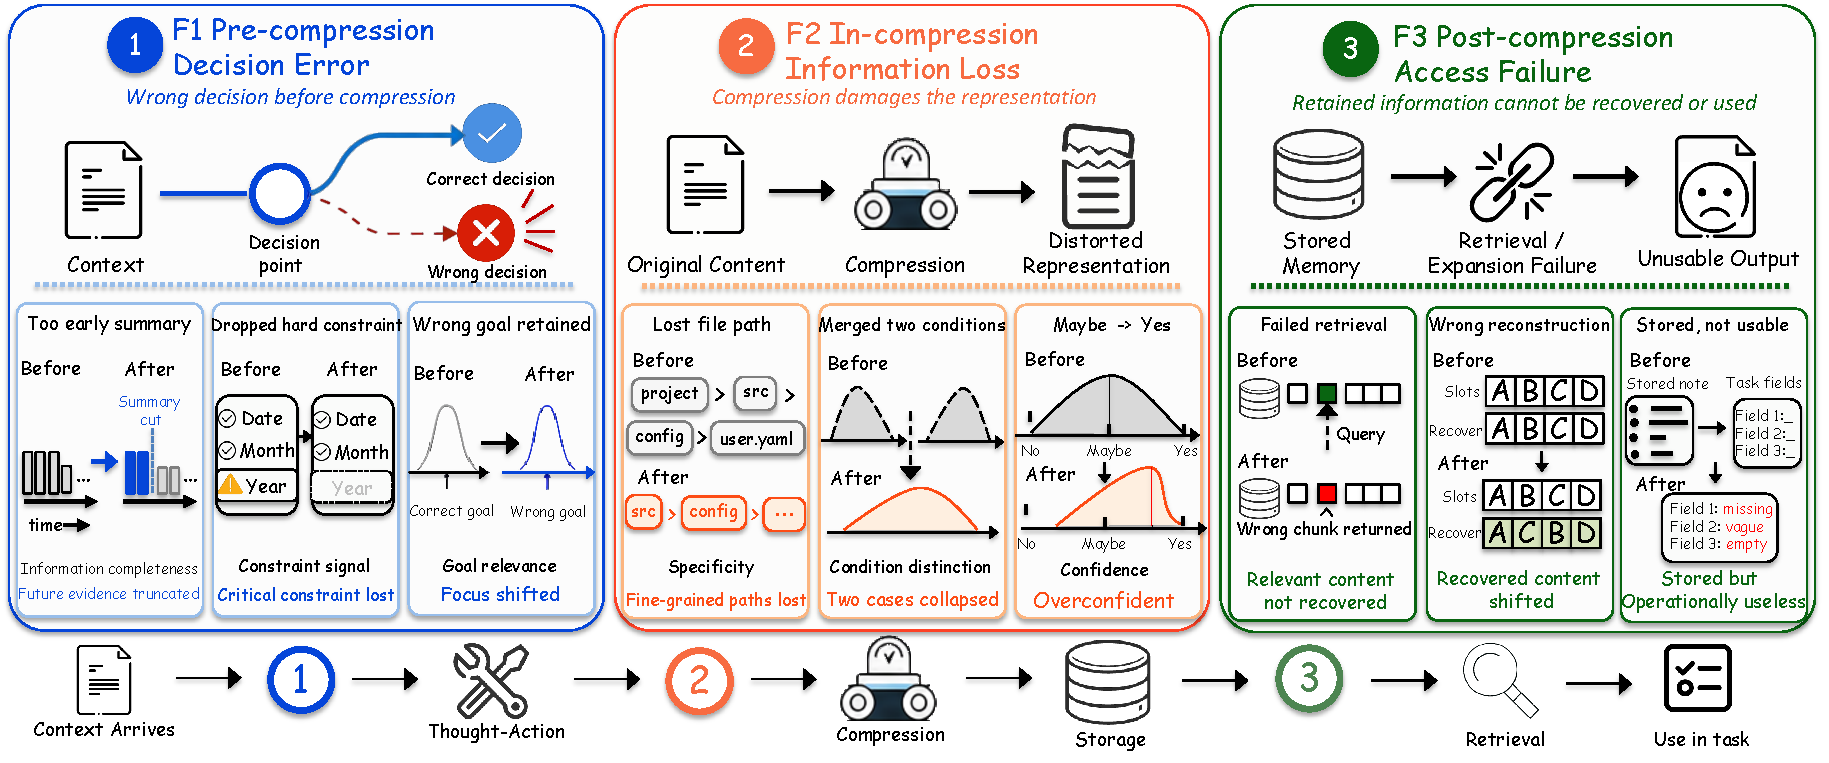
\includegraphics[width=0.85\textwidth]{figures/section5.pdf}
%     \caption{A temporal taxonomy of context compression failures. Failures are classified by the earliest point at which they occur in the compression pipeline: {\fone}, {\ftwo}, and {\fthree}.}
%     \label{fig:failure_modes_taxonomy}
% \end{figure*}

% \paragraph{\fone} refers to failures arising before compression is performed, where the system makes incorrect decisions regarding whether to compress, when to compress, what information should be compressed, and at what granularity compression should occur. The core issue in this category does not lie in the correctness of the compression operation itself, but rather in the fact that the upstream decision-making process has already deviated from task requirements. Typical examples include compressing information prematurely~\citep{yang2026staticsummarizationproactivememory, liu2025contexttoolcontextmanagement}, misjudging the retention value of critical information~\citep{liang2026learningremembermetacognitivemanagement, feng2026agentocrreimaginingagenthistory}, or incorporating core constraints that should remain intact into the compression process~\citep{liu2025contexttoolcontextmanagement}, thereby leading to subsequent information loss or contextual mismatch during execution.

% \paragraph{\ftwo} refers to failures in which the compression operation itself causes information corruption during the process of representation transformation, resulting in substantial loss of the original content’s semantics, structure, relationships, constraints, or fine-grained details in the compressed representation. The core issue in this category does not concern whether the pre-compression decision was appropriate, but rather whether the compression process faithfully preserves the original information. Typical examples include the omission of critical semantics~\citep{chen2026halumemevaluatinghallucinationsmemory, yang2026staticsummarizationproactivememory}, the disruption of relational structures~\citep{wu2026contextweaverselectivedependencystructuredmemory}, the over-simplification of constraint conditions~\citep{chen2026halumemevaluatinghallucinationsmemory, liu2025contexttoolcontextmanagement}, or the erroneous compression of uncertainty in the original content into overly definitive conclusions~\citep{yang2026staticsummarizationproactivememory}, thereby preventing the compressed representation from fully supporting subsequent reasoning and execution.

% \paragraph{\fthree} refers to failures in which compressed information has technically been retained in some form, yet cannot be correctly retrieved, accessed, expanded, or reconstructed during subsequent use. The core issue in this category lies neither in whether the pre-compression decision was appropriate nor in whether the compression process itself introduced information corruption, but rather in failures of post-compression accessibility and recoverability. Typical examples include situations where information still exists but cannot be successfully retrieved~\citep{li2026ocrmemoryopticalcontextretrieval, zeng2026kvcachecentric, chen2026halumemevaluatinghallucinationsmemory}, where retrieved information is reconstructed incorrectly~\citep{chen2026halumemevaluatinghallucinationsmemory}, or where the compressed representation remains formally storable yet functionally unusable~\citep{li2026ocrmemoryopticalcontextretrieval, zeng2026kvcachecentric}, thereby preventing the originally preserved content from being effectively utilized in downstream tasks.

% In summary, \ensuremath{F^{1}}–\ensuremath{F^{3}} collectively constitute a complete causal chain of context compression failures in temporal order. The three categories are naturally distinguished by their positions within the failure pipeline. By classifying each failure according to the earliest and most critical point at which the error occurs, the framework can maintain both mutual exclusivity and overall completeness. For hybrid cases involving multiple issues simultaneously, priority should be given to annotating the earliest failure source that causally triggers subsequent errors, since agent workflows inherently exhibit error propagation characteristics~\citep{wang2024survey}.

% We organize context compression failures by the earliest stage at which they arise: {\fone}, {\ftwo}, and {\fthree}, as shown in Figure~\ref{fig:failure_modes_taxonomy}.

% \begin{figure*}[t]
%     \centering
%     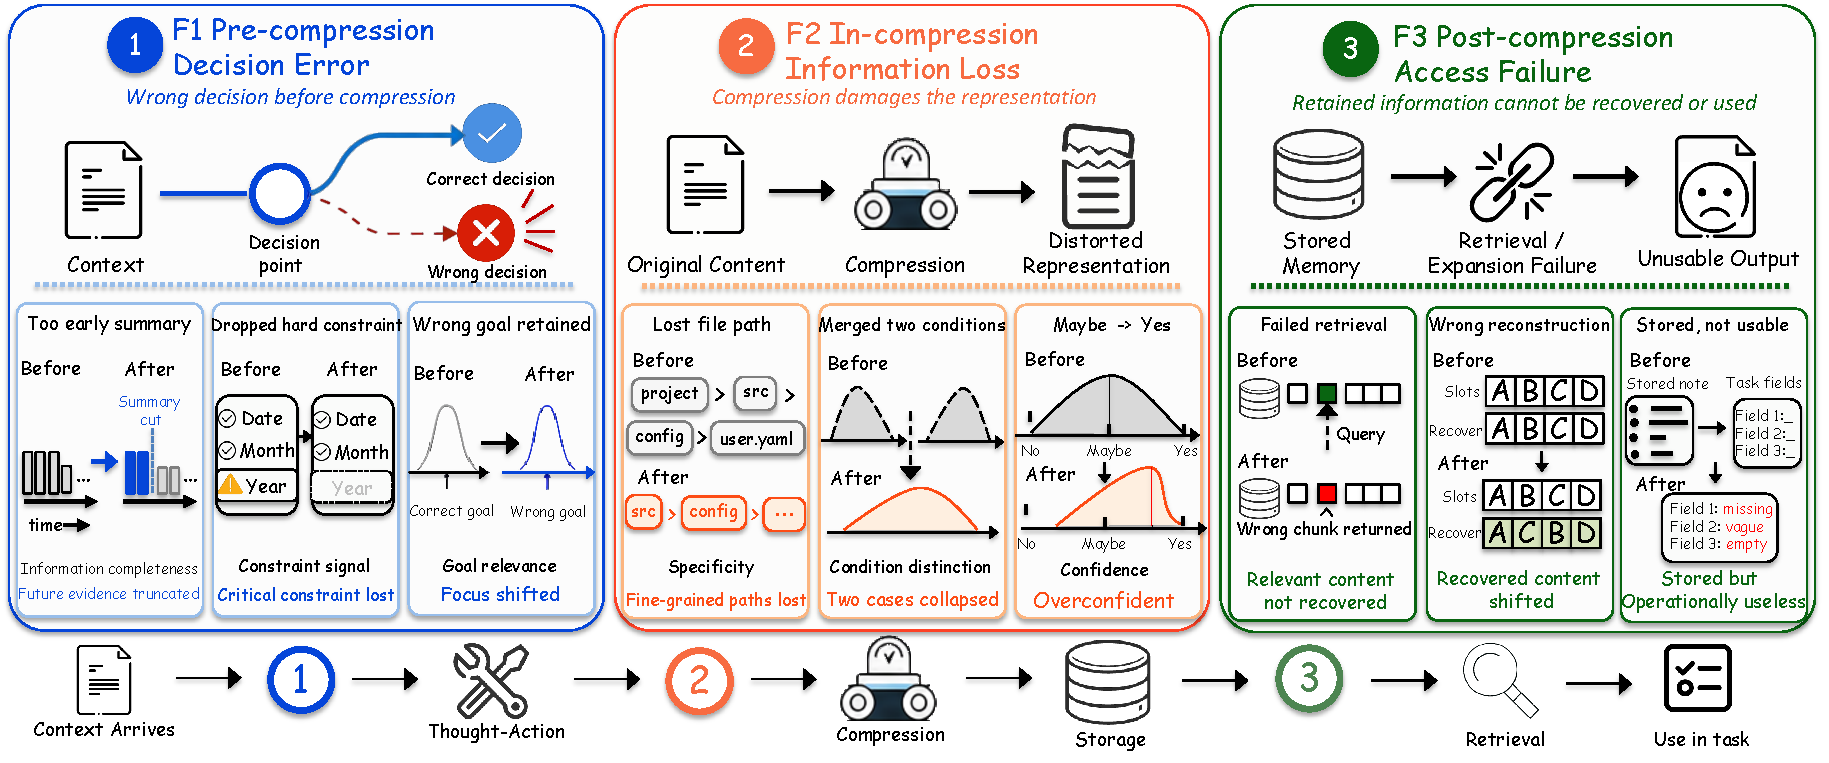
\includegraphics[width=0.75\textwidth]{figures/section5.pdf}
%     \vspace{-.2cm}
%     \caption{A temporal taxonomy of context compression failures. Failures are classified by the earliest point at which they occur in the compression pipeline: {\fone}, {\ftwo}, and {\fthree}.}
%     \label{fig:failure_modes_taxonomy}
% \end{figure*}

% \begin{figure*}[ht]
%     \centering
%     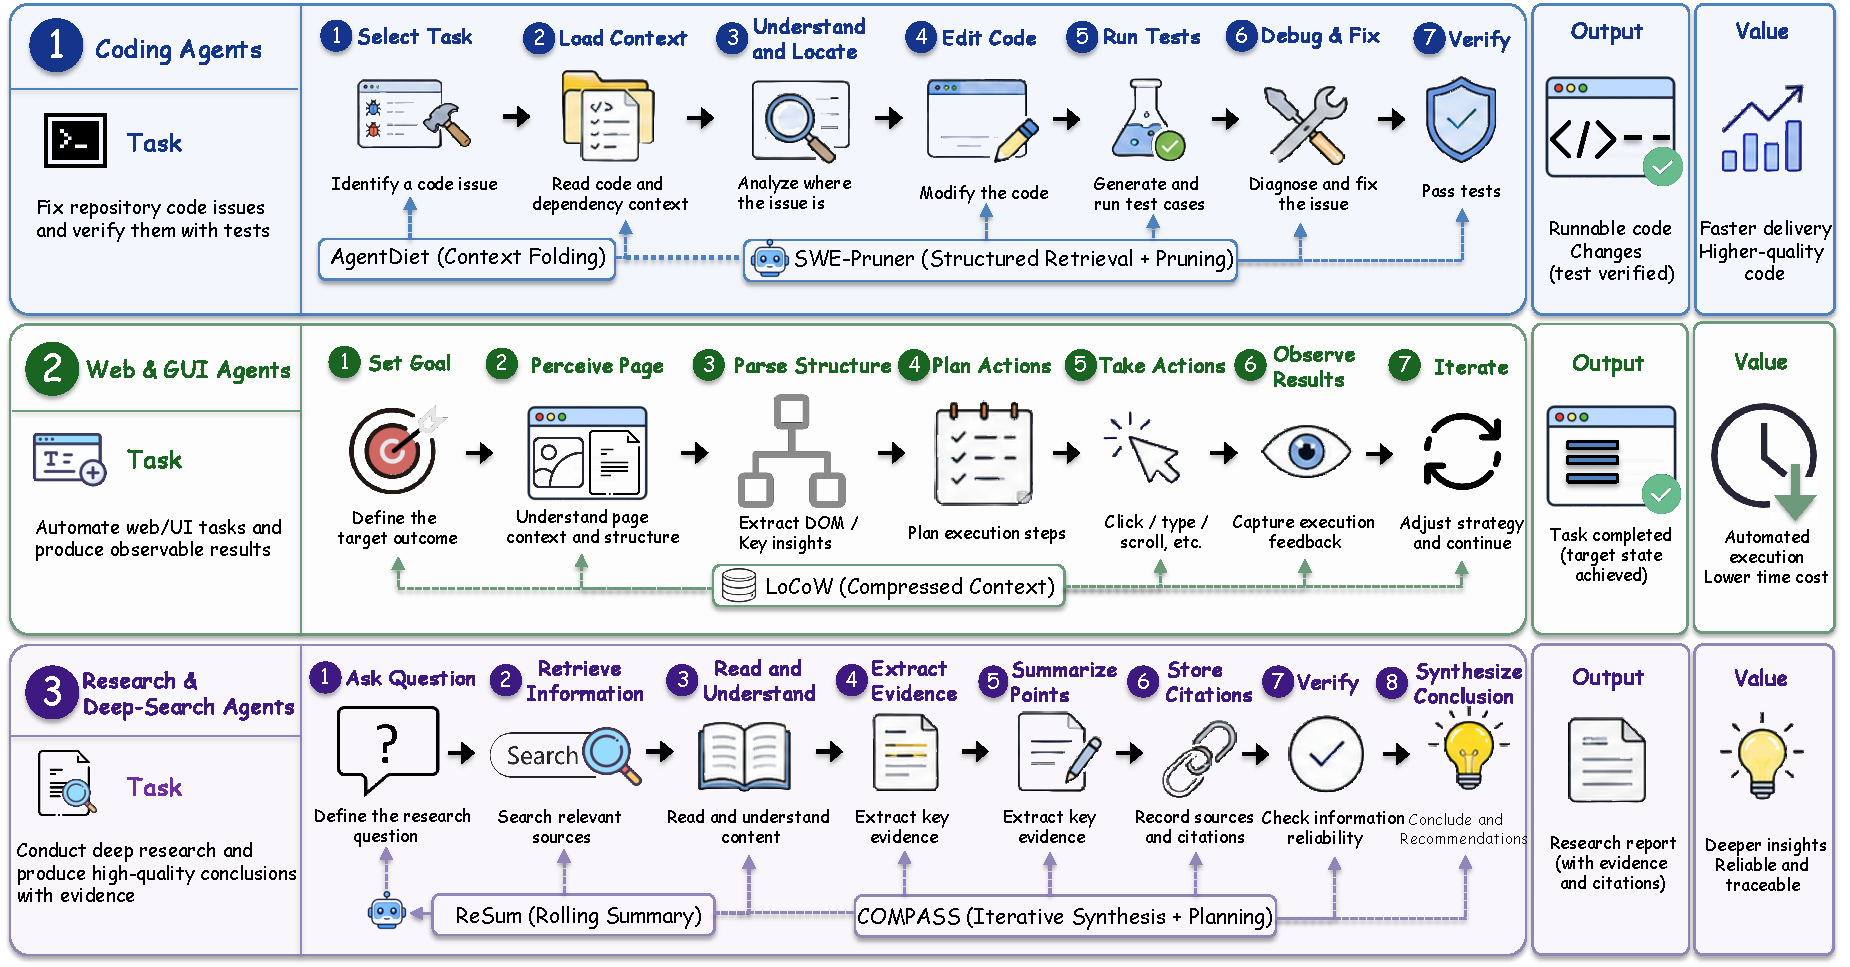
\includegraphics[width=0.8\textwidth]{figures/section6.pdf}
%      \vspace{-.2cm}
%     \caption{Domain-specific context compression regimes for coding, web/GUI, and research agents. The figure contrasts each domain's setup, workflow, interaction loop, dominant risks, and contextualized strategy choices.}
%     \label{fig:domain_specific_regimes}
% \end{figure*}

% \begin{table*}[ht]
% \centering
% \footnotesize
% \setlength{\tabcolsep}{4pt}
% \setlength{\aboverulesep}{0.2ex}
% \setlength{\belowrulesep}{0.2ex}
% \renewcommand{\arraystretch}{0.98}
% \begin{tabularx}{\textwidth}{@{}>{\raggedright\arraybackslash}p{2.2cm} >{\raggedright\arraybackslash}X >{\raggedright\arraybackslash}X >{\raggedright\arraybackslash}X >{\raggedright\arraybackslash}X@{}}
% \toprule
% \textbf{System} & \textbf{Select ($S$)} & \textbf{Compress ($\Phi$)} & \textbf{Store ($M$)} & \textbf{Recover ($R$)} \\
% \midrule
% \textbf{Claude Code} & Reactive, threshold-based selection. & Auto-compaction of prior interaction history. & Compacted state retained in active context. & Implicit recovery via continued execution. \\
% \midrule
% \textbf{Cursor} & Retrieval-first selection of files, code blocks, and rules. & Relevance filtering and contextual assembly. & Repository index, project rules, and workspace context. & Re-injection of retrieved files, rules, and evidence. \\
% \midrule
% \textbf{OpenAI Codex} & Task-grounded selection over files, instructions, and threads. & Session continuation and workspace grounding. & Task threads, instruction files, and repository state. & Recovery through continued threads and file re-access. \\
% \bottomrule
% \end{tabularx}
% \caption{Pipeline-level comparison of recent production-grade coding agents, organized by the stages in Section~\ref{subsec:unified_pipeline}.}
% \label{tab:coding_agents_pipeline}
% \end{table*}

% \noindent\textbf{\fone} refers to failures that arise before compression itself, when the system chooses the wrong moment, target, or granularity of compression. The issue is not the compression operator, but a pre-compression decision that already departs from task requirements. Typical cases include premature compression~\citep{yang2026staticsummarizationproactivememory, liu2025contexttoolcontextmanagement}, misjudging the retention value of critical information~\citep{liang2026learningremembermetacognitivemanagement, feng2026agentocrreimaginingagenthistory}, or compressing constraints that should remain exact~\citep{liu2025contexttoolcontextmanagement}. Appendix~\ref{app:case-studies-compression-failures} illustrates this pattern with a case where a compression controller prematurely removes authentication-related state before the agent reaches the step where it is required.

% \noindent\textbf{\ftwo} refers to failures introduced by the compression operation itself, where representation transformation corrupts semantics, structure, relations, constraints, or fine-grained detail. The central question is whether compression preserves the original information faithfully enough for later use. Typical cases include omitted semantics~\citep{chen2026halumemevaluatinghallucinationsmemory, yang2026staticsummarizationproactivememory}, disrupted relational structure~\citep{wu2026contextweaverselectivedependencystructuredmemory}, oversimplified constraints~\citep{chen2026halumemevaluatinghallucinationsmemory, liu2025contexttoolcontextmanagement}, or compressed uncertainty that becomes an unwarranted conclusion~\citep{yang2026staticsummarizationproactivememory}. Appendix~\ref{app:case-studies-compression-failures} provides a trajectory-level example in which compression preserves the broad task intent but loses a fine-grained constraint, causing the later agent state to become semantically incomplete.

% \noindent\textbf{\fthree} refers to failures of post-compression accessibility: information is retained in some form, but cannot be correctly retrieved, expanded, or reconstructed when needed. The issue is therefore recoverability rather than pre-compression choice or in-compression corruption. Typical cases include failed retrieval~\citep{li2026ocrmemoryopticalcontextretrieval, zeng2026kvcachecentric, chen2026halumemevaluatinghallucinationsmemory}, incorrect reconstruction~\citep{chen2026halumemevaluatinghallucinationsmemory}, or compressed states that remain storable yet functionally unusable~\citep{li2026ocrmemoryopticalcontextretrieval, zeng2026kvcachecentric}. Appendix~\ref{app:case-studies-compression-failures} shows the corresponding access-side failure: the correct compressed memory exists, but later retrieval returns a semantically similar yet wrong memory item.

% Together, \textbf{F1}–\textbf{F3} define a temporal failure taxonomy over the compression pipeline. For hybrid cases, we assign the label to the earliest failure that causally triggers later errors, since agent workflows naturally exhibit error propagation~\citep{wang2024survey}.


% % We synthesized the existing literature on context compression failure modes and organized them into an exhaustive and non-overlapping taxonomy along the temporal sequence of compression, which are {\fone}, {\ftwo} and {\fthree}, respectively, as illustrated in Figure~\ref{fig:failure_modes_taxonomy}.

% % \begin{figure*}[t]
% %     \centering
% %     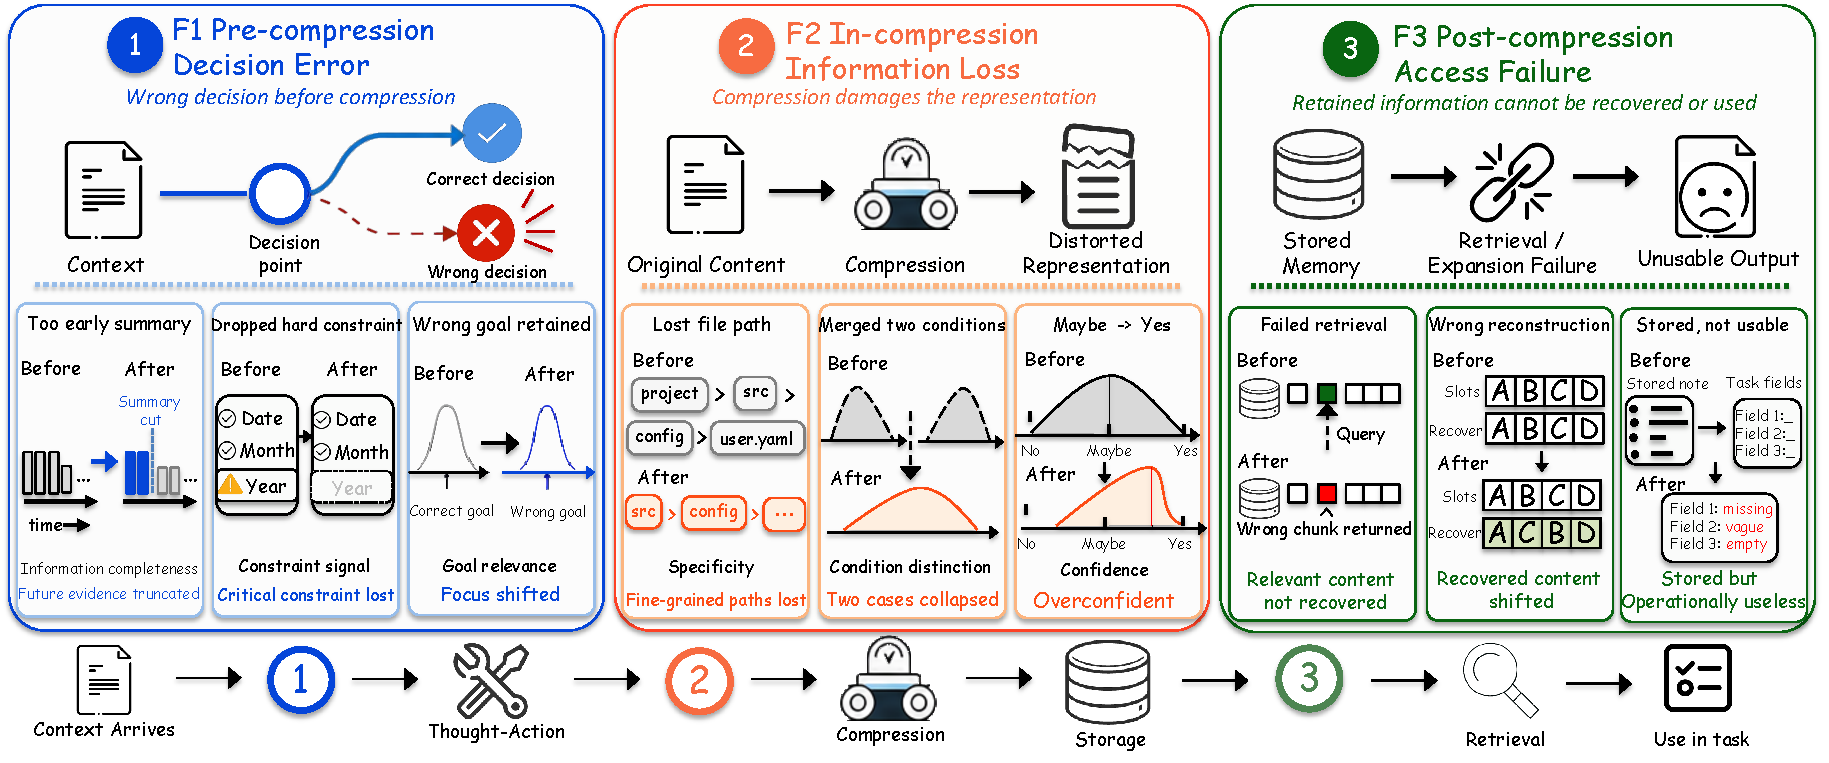
\includegraphics[width=0.85\textwidth]{figures/section5.pdf}
% %     \caption{A temporal taxonomy of context compression failures. Failures are classified by the earliest point at which they occur in the compression pipeline: {\fone}, {\ftwo}, and {\fthree}.}
% %     \label{fig:failure_modes_taxonomy}
% % \end{figure*}

% % \paragraph{\fone} refers to failures arising before compression is performed, where the system makes incorrect decisions regarding whether to compress, when to compress, what information should be compressed, and at what granularity compression should occur. The core issue in this category does not lie in the correctness of the compression operation itself, but rather in the fact that the upstream decision-making process has already deviated from task requirements. Typical examples include compressing information prematurely~\citep{yang2026staticsummarizationproactivememory, liu2025contexttoolcontextmanagement}, misjudging the retention value of critical information~\citep{liang2026learningremembermetacognitivemanagement, feng2026agentocrreimaginingagenthistory}, or incorporating core constraints that should remain intact into the compression process~\citep{liu2025contexttoolcontextmanagement}, thereby leading to subsequent information loss or contextual mismatch during execution.

% % \paragraph{\ftwo} refers to failures in which the compression operation itself causes information corruption during the process of representation transformation, resulting in substantial loss of the original content’s semantics, structure, relationships, constraints, or fine-grained details in the compressed representation. The core issue in this category does not concern whether the pre-compression decision was appropriate, but rather whether the compression process faithfully preserves the original information. Typical examples include the omission of critical semantics~\citep{chen2026halumemevaluatinghallucinationsmemory, yang2026staticsummarizationproactivememory}, the disruption of relational structures~\citep{wu2026contextweaverselectivedependencystructuredmemory}, the over-simplification of constraint conditions~\citep{chen2026halumemevaluatinghallucinationsmemory, liu2025contexttoolcontextmanagement}, or the erroneous compression of uncertainty in the original content into overly definitive conclusions~\citep{yang2026staticsummarizationproactivememory}, thereby preventing the compressed representation from fully supporting subsequent reasoning and execution.

% % \paragraph{\fthree} refers to failures in which compressed information has technically been retained in some form, yet cannot be correctly retrieved, accessed, expanded, or reconstructed during subsequent use. The core issue in this category lies neither in whether the pre-compression decision was appropriate nor in whether the compression process itself introduced information corruption, but rather in failures of post-compression accessibility and recoverability. Typical examples include situations where information still exists but cannot be successfully retrieved~\citep{li2026ocrmemoryopticalcontextretrieval, zeng2026kvcachecentric, chen2026halumemevaluatinghallucinationsmemory}, where retrieved information is reconstructed incorrectly~\citep{chen2026halumemevaluatinghallucinationsmemory}, or where the compressed representation remains formally storable yet functionally unusable~\citep{li2026ocrmemoryopticalcontextretrieval, zeng2026kvcachecentric}, thereby preventing the originally preserved content from being effectively utilized in downstream tasks.

% % In summary, \ensuremath{F^{1}}–\ensuremath{F^{3}} collectively constitute a complete causal chain of context compression failures in temporal order. The three categories are naturally distinguished by their positions within the failure pipeline. By classifying each failure according to the earliest and most critical point at which the error occurs, the framework can maintain both mutual exclusivity and overall completeness. For hybrid cases involving multiple issues simultaneously, priority should be given to annotating the earliest failure source that causally triggers subsequent errors, since agent workflows inherently exhibit error propagation characteristics~\citep{wang2024survey}.


\section{Domain-Specific Analysis}
\label{sec:5_domain_specific_analysis}


Compression is domain-dependent: coding agents require structural fidelity and state continuity; web and GUI agents must preserve heterogeneous multimodal observations; DeepResearch agents depend on deferred evidence recovery across long horizons. Figure~\ref{fig:domain_specific_regimes} summarizes these regimes.

% The practical value of a compression strategy is domain-dependent. Coding agents require high structural fidelity and explicit state continuity; web and GUI agents face heterogeneous multimodal observations; research agents depend most on deferred evidence recovery across long horizons. Figure~\ref{fig:domain_specific_regimes} summarizes these regimes.


\noindent\textbf{Coding Agents}
Coding places the strongest pressure on structure preservation, exact evidence retention, and reliable recovery. Accordingly, methods such as SWE-Pruner~\citep{wang2026sweprunerselfadaptivecontextpruning}, LongCodeZip~\citep{shi2025longcodezip}, and CAT~\citep{liu2025contexttoolcontextmanagement} emphasize structure-aware pruning and explicit state retention.
Table~\ref{tab:coding_agents_pipeline} compares recent production-grade coding agents through the unified operational pipeline, using only public evidence and high-confidence product signals.
The contrast is instructive. Claude Code emphasizes \textbf{Compress} through reactive compaction, Cursor places more weight on \textbf{Store} and \textbf{Recover} through repository indexing and retrieval, and Codex appears most grounded in \textbf{Select} plus workspace continuation. Across all three, the common pattern is not aggressive lossy shortening, but coordinated pipeline control under tight context budgets.


\noindent\textbf{Web \& GUI Agents}
Web and GUI agents operate over heterogeneous, partially redundant observations. Methods such as LCoW~\citep{lee2025learningcontextualizewebpages} and PAL-UI~\citep{liu2025paluiplanningactivelookback} exploit redundancy, but representation-level compression must still preserve modality and interface cues.

\noindent\textbf{DeepResearch  Agents}
Research and deep-search agents are defined less by structural fidelity than by delayed evidence use. Their main risk is that abstraction hides evidence that matters only later. ReSum~\citep{wu2026resumunlockinglonghorizonsearch} and COMPASS~\citep{wan2025compassenhancingagentlonghorizon} favor summarization, whereas Step-DeepResearch~\citep{hu2025stepdeepresearchtechnicalreport} and WebWeaver~\citep{li2025webweaverstructuringwebscaleevidence} externalize or retrieve evidence to preserve long-horizon dependencies.



% \input{tables/5_evaluation_dimensions}
\section{Beyond Task Success: Rethinking Evaluation}
\label{sec:6_evaluation}
% We reframe evaluation of agent context compression as a metric system over the compression target, rather than as a loose discussion of downstream performance. Let the compressed context state be defined by four components: \(Q=(D,R,P,O)\), where \(D\) denotes task-relevant density, \(R\) recoverability, \(P\) propagation of compression error, and \(O\) operational overhead. Under this view, a method is preferred when it maximizes useful preservation and recoverability while minimizing error spread and control cost.

% Equivalently, we can express the evaluation objective as \(J=\alpha D+\beta R-\gamma P-\delta O\), where the weights reflect the priorities of the target domain and agent setting. This formulation makes comparison more explicit: methods should not only be judged by final task success, but by how well they preserve information, support restoration, limit long-horizon failure, and remain efficient under budget constraints.

% Therefore, the objective \(J\) provides the comparison criterion for this section, linking benchmark results to compression quality under the domain-specific constraints \(\mathrm{Constraint}_i\).
\noindent\textbf{Outcome-Centric Evaluation.}
Benchmarks still judge context compression mainly by downstream task success. Success rate, with token count or compression ratio as an auxiliary proxy, remains the default protocol. This is convenient but inadequate: success entangles compression with planning and execution, while shorter prompts reveal little about whether task-critical evidence survives. Cross-paper comparison is further blurred by changes in backbone, task set, and context budget.

% \noindent\textbf{Current practice.}
% Current benchmarks treat context compression mainly as an ingredient of downstream task performance. Success rate, with token count or compression ratio as a secondary proxy, remains the default protocol. This is convenient but fundamentally insufficient: task success conflates compression with planning and execution, while shorter prompts say little about how much task-relevant information remains. Cross-paper comparison is further weakened by changes in agent backbone, task set, and context budget.

\noindent\textbf{The Missing Object.} The missing object is not the task outcome but the compressed state itself. For agents, four dimensions are decisive: \textit{information density}, \textit{recoverability}, \textit{error propagation}, and \textit{controller overhead}. Together, they ask whether compression preserves task-critical evidence, supports later restoration, avoids long-horizon failure amplification, and remains efficient enough to justify its control cost.

% \noindent\textbf{What is missing.} The missing object of evaluation is the compressed state itself. For agents, four dimensions are decisive: \textit{information density}, \textit{recoverability}, \textit{error propagation}, and \textit{controller overhead}. Together, they ask whether compression preserves task-critical evidence, supports later restoration, avoids long-horizon failure amplification, and remains efficient enough to justify its own control cost.

\noindent\textbf{From Outcomes to State Quality.} We therefore evaluate compressed states through \(Q=(D,R,P,O)\), where \(D\) denotes task-relevant density, \(R\) recoverability, \(P\) propagation risk, and \(O\) operational overhead, and summarize comparison through \(J=\alpha D+\beta R-\gamma P-\delta O\). The point is simple but consequential: compression should be judged as state quality, not only task outcome. This reframing ties benchmark outcomes to compression quality under domain-specific constraints \(\mathrm{Constraint}_i\).
% \noindent\textbf{A sharper framework.}  We therefore evaluate a compressed state through \(Q=(D,R,P,O)\), where \(D\) denotes task-relevant density, \(R\) recoverability, \(P\) propagation risk, and \(O\) operational overhead, and summarize comparison through \(J=\alpha D+\beta R-\gamma P-\delta O\). The core shift is conceptual: evaluation should treat compression as a state-quality problem, not merely an outcome-only scoring problem. This reframing links benchmark outcomes back to compression quality under domain-specific constraints \(\mathrm{Constraint}_i\).
Taken together, this reframing motivates a broader discussion of recoverable, faithful, and long-horizon context management, which we defer to Appendix~\ref{ap:extended_future_directions}.
% Taken together, these directions point toward a broader concluding discussion on recoverable, faithful, and long-horizon context management, which we defer to Appendix~\ref{ap:extended_future_directions}.




% \section{Open Problems \& Future Directions}
% \label{sec:7_future_directions}
% \paragraph{Compression, retrieval, and memory} should be treated as distinct but coupled design choices. A clearer framework is still needed to decide when information should remain in active context, when it should be compressed, and when it should be externalized for later recovery.

\paragraph{Recoverable and adaptive compression} remains the central technical challenge. Future methods should optimize not only task success and token efficiency, but also whether compressed information can be reconstructed when needed and whether compression behavior remains aligned with long-horizon execution.

\paragraph{Benchmarks and methods must become more domain-aware.} As shown in \S~\ref{sec:5_domain_specific_analysis}, coding, web/GUI, and research agents impose different requirements on fidelity, recoverability, and evidence precision. Progress will therefore require both domain-specific compression strategies and standardized benchmarks that measure compressed-state quality beyond task success.



\section{Conclusion}
\label{sec:8_conclusion}

Agent context compression is no longer just a preprocessing convenience. For long-horizon agents, it is a state-management problem over a changing workspace, not a one-shot prompt-shortening step. This survey structures the area along three axes: targets, mechanisms, and control policies. It also introduces a failure taxonomy and an evaluation framework that goes beyond task success. The key challenge is not only stronger compression, but compression that remains recoverable, faithful, and aligned with long-term agent execution.


\section*{Limitations}
\label{sec:limitations}
% This survey has several scope limitations. First, because agent context compression is evolving rapidly, our synthesis is necessarily representative rather than permanently exhaustive, especially for very recent systems and unpublished engineering practices. Second, we focus on application-level context management during agent execution, and therefore do not attempt a full treatment of neighboring areas such as general long-context modeling, model-level KV-cache optimization, or broader memory architectures except where they directly inform agent compression. Third, our taxonomy prioritizes conceptual unification across targets, mechanisms, policies, failure modes, and evaluation, which improves comparability but cannot fully eliminate heterogeneity in backbone models, task settings, and reporting protocols across the literature. We view these limitations as a consequence of studying a fast-moving systems problem, and hope the framework provided here offers a stable foundation for more exhaustive benchmarked updates as the field matures.

\paragraph{Coverage.} Because agent context compression is evolving rapidly, our synthesis is intended to be representative rather than exhaustive, especially for the newest systems and engineering practices still stabilizing in the literature.

\paragraph{Scope.} We deliberately focus on context compression during agent execution, rather than adjacent areas such as general long-context modeling, context engineering, memory management, or model-level KV-cache optimization, except where they directly inform agent compression. We view these neighboring directions as natural extensions and leave a unified treatment to future work.

\paragraph{Abstraction Level.} Our taxonomy prioritizes conceptual unification across targets, mechanisms, policies, failure modes, and evaluation. This improves comparability, but necessarily abstracts away some implementation-level variation across backbone models, task settings, and reporting protocols.

We view these limitations primarily as boundaries of scope rather than weaknesses of the framework, and hope the structure offered here provides a stable basis for more exhaustive updates as the field matures.



\section*{AI Usage Disclosure}
The authors used AI-based writing assistants to improve grammar, phrasing, and local clarity during manuscript preparation. All AI-assisted suggestions were reviewed, revised, and selectively incorporated by the authors, who take full responsibility for the final text, technical framing, citations, and conclusions.

\section*{Ethical Statement}
This work is a survey of publicly available research papers, technical reports, product documentation, and open-source resources on context management for LLM agents. It does not involve private data, human subjects, or sensitive personal information. We aim to represent prior work accurately and cite sources faithfully; any discussion of deployed systems is based only on publicly accessible evidence and is used solely for scholarly analysis.



% Bibliography entries for the entire Anthology, followed by custom entries
%\bibliography{custom,anthology-overleaf-1,anthology-overleaf-2}

% Custom bibliography entries only
\bibliography{custom}

\appendix

\newpage

\section{Methodology of the Survey}
\label{app:methodology}

\subsection{Search Strategy}
\label{app:search-strategy}

Because agent context compression is an emerging topic without a unified terminology, we adopted a broad search strategy rather than relying on a single keyword. We searched ACL Anthology, DBLP, arXiv, Google Scholar, Semantic Scholar, and major NLP, machine learning, software engineering, and agent-system venues. The search covered both explicit compression terms and adjacent terms used in related communities.

Specifically, we used keyword combinations such as \textit{``LLM agent''} with \textit{``context compression''}, \textit{``trajectory compression''}, \textit{``history summarization''}, \textit{``context pruning''}, \textit{``context folding''}, \textit{``agent memory compression''}, \textit{``memory retrieval''}, and \textit{``long-horizon agent context''}. We also searched domain-specific terms, including \textit{``coding agent context''}, \textit{``web agent memory''}, \textit{``GUI agent observation compression''}, and \textit{``deep research agent memory''}. These queries were designed to capture papers that may not use the exact phrase \textit{context compression} but nevertheless reduce, rewrite, externalize, or retrieve agent history under a limited context budget.

In addition to keyword search, we performed backward and forward citation tracing from representative work on prompt compression, long-context modeling, agent memory, web agents, coding agents, and deep-research agents. This step was necessary because many relevant systems describe compression-related operations as \textit{memory management}, \textit{state retention}, \textit{context engineering}, \textit{trajectory summarization}, or \textit{retrieval-based continuation}. We therefore treated terminology flexibly and focused on whether a method changes what historical information remains available to the agent during future execution.

\subsection{Inclusion and Exclusion Criteria}
\label{app:inclusion-exclusion}

We included a paper or system if it satisfied at least one of the following conditions. First, it proposes a method that compresses, filters, summarizes, prunes, folds, externalizes, or retrieves the context of an LLM agent during multi-step execution. Second, it introduces a memory or retrieval mechanism whose purpose is to preserve task-relevant information under a finite context budget. Third, it analyzes long-horizon agent behavior in a way that reveals failures caused by context reduction, memory selection, retrieval, or compressed-state reuse. Fourth, it describes a deployed or production-grade agent system with publicly documented context-management behavior relevant to the operational pipeline studied in this survey.

We excluded work whose primary contribution lies outside application-level agent context management. In particular, we excluded methods that only compress static, single-turn prompts unless they are explicitly adapted to multi-step agent trajectories. We also excluded model-level compression methods, such as weight quantization, model pruning, distillation, and generic KV-cache optimization, when they do not alter the information available to the agent as part of its executable context. Similarly, general retrieval-augmented generation was not treated as agent context compression unless retrieval is coupled to an evolving agent state, trajectory history, or memory store.

For borderline cases, we used a functional criterion: a work was considered relevant if its method changes how past observations, actions, thoughts, plans, or memory states are preserved and reused for future decisions under a context constraint. This criterion allowed us to include systems that do not explicitly use the term \textit{compression} but still perform compression-like state management. When a method combined multiple components, such as summarization plus retrieval or pruning plus external memory, we categorized it according to the component that most directly determines the compressed state available to later agent execution.

Finally, for production-grade systems and technical reports, we only relied on public evidence and high-confidence descriptions. When implementation details were unavailable, we characterized the system at the level of observable pipeline behavior rather than making assumptions about proprietary mechanisms.


\section{Extended Taxonomies and Resources}
\label{ap:extended_taxonomies}

\subsection{Details about taxonomy}
\label{ap:details_about_taxonomy}
In the main text, we characterize context management methodologies based on three core dimensions, specifically \textit{when}, \textit{what}, and \textit{how}, while further analyzing their application \textit{domain} as a complementary perspective. Table~\ref{tab:full_taxonomy} below instantiates this framework at the level of individual methods. Specifically, the \textit{when} column indicates the trigger mechanism and decision maker for context compression or management, including system-controlled, external-controller, agent-controlled, and learned policies; the \textit{what} column identifies the context object being managed, such as observations, trajectories, memory states, plans and reasoning traces, or representation-level signals; and the \textit{how} column summarizes the compression mechanism, including truncation and masking, pruning and reduction, summarization and abstraction, externalization and retrieval, and representation-level compression. In addition to these three dimensions, we report the \textit{domain} of each method to indicate its primary task setting, and we analyze its distribution and characteristics separately in the main text. Taken together, the table provides a fine-grained view of how different methods are positioned within the taxonomy and how their design choices vary across task domains.

\subsection{Open-Source Standouts}
\label{ap:open_source_standouts}
To more comprehensively reflect the openness and reproducibility of research in this area, we further collected and summarized the open-source methods included in this survey, as shown in Table~\ref{tab:opensource_methods}. The table exclusively incorporates methods accompanied by publicly available code, presenting them across three columns: method name, open-source link, and publication year. This organization enables readers to efficiently locate the corresponding implementations and repository resources. As shown in the table, the current open-source work is concentrated in a small number of representative methods, and the release years span 2025 to 2026, which indicates that this field is still evolving rapidly and that its open-source ecosystem is steadily maturing. Overall, this statistics not only improves the reproducibility of our survey results, but also provides a direct entry point for future researchers to conduct method comparison, code replication, and further development.

\subsection{Datasets \& Benchmarks}
Table~\ref{tab:datasets_benchmarks} summarizes the representative datasets and benchmarks collected in \texttt{datasets\_info.md}. We organize them by task family and retain only the information most useful for a survey on agentic context management: benchmark purpose, publication venue/year, and public availability. To keep the table compact, we move the task-focus and scale description into the benchmark cell itself, so each row reads as a short self-contained summary.

The \emph{Benchmark} cell includes the dataset name, a citation to the original paper, and a brief description of the task and scale. The \emph{Source and year} column records the original publication venue or release year, while the \emph{Open Source} column provides the public repository or dataset URL when available, and indicates the absence of public releases otherwise. Benchmarks with closely related variants are grouped together to keep the presentation compact.

First, the selected benchmarks are intentionally diverse, encompassing software engineering, web browsing, office automation, mobile apps, deep research, long-context reasoning, memory, code generation, and long-document summarization. This diversity is essential, as context management methods frequently navigate the trade-off between retaining essential task-critical evidence and pruning redundant historical data, with individual benchmarks typically evaluating only a specific subset of these behaviors.

Second, numerous benchmarks are structured as closely related families or variants. For instance, \emph{SWE-bench Verified}~\citep{jimenez2024swebench} and \emph{SWE-bench Lite}~\citep{jimenez2024swebench} assess software issue resolution under different difficulty and edit constraints; \emph{BrowseComp}~\citep{wei2025browsecomp}, \emph{BrowseComp-Plus}~\citep{chen2025browsecompplus}, and \emph{BrowseComp-ZH}~\citep{zhou2025browsecompzh} cover browsing-centric deep search in different settings; \emph{Mind2Web}~\citep{deng2023mind2web} and \emph{Multimodal-Mind2Web}~\citep{zheng2024seeact} differ by adding visual grounding; \emph{LongBench}~\citep{bai2024longbench}, \emph{LongBench V2}~\citep{bai2025longbenchv2}, \emph{BABILong}~\citep{NEURIPS2024_babilong}, \emph{NeedleBench}~\citep{li2024needlebench}, and \emph{NIAH}~\citep{liu2023lost} probe long-context handling from complementary angles.

Third, in instances where a benchmark entry represents a comprehensive framework or family rather than an isolated dataset, we designate it by its representative name in the table and elucidate the included variants within the accompanying notes. This is especially helpful for benchmarks such as \emph{MRQA}~\citep{fisch-etal-2019-mrqa}, \emph{Loghub}~\citep{zhu2023loghub}, and \emph{CompileBench / CRUST-Bench}~\citep{khatry2025crustbench}, where a single umbrella name aggregates multiple sub-datasets or tasks.

Finally, the \emph{Open Source} column is interpreted broadly, providing the public dataset or repository URL when available, and explicitly noting cases where no public release could be identified within the collected sources. The original publication year and venue are preserved in the \emph{Source and year} column.


\section{Implementation Details of Compression Operators}
\label{app:operator-details}

This appendix supplements the taxonomy in Section~\ref{subsec:compression_mechanism} by summarizing concrete implementation details of representative compression operators. We focus on three methods with relatively explicit descriptions: ReSum \citep{wu2026resumunlockinglonghorizonsearch} and AgentFold  \citep{ye2025agentfoldlonghorizonwebagents} for summarization and abstraction, and SWE-Pruner \citep{wang2026sweprunerselfadaptivecontextpruning} for pruning and reduction. The goal is not to reproduce full prompts verbatim, but to identify the prompt roles, response templates, algorithmic steps, and compression-specific design choices that instantiate the operator families discussed in the main text.

\subsection{Prompts for Summarization and Abstraction}
\label{app:prompts-summarization}

Summarization and abstraction methods rewrite long interaction histories into shorter executable states. Table~\ref{tab:app-c1-prompts} compares the concrete prompt or response-template designs in ReSum and AgentFold. ReSum exposes summarization as a separate tool invocation that periodically converts a growing trajectory into a compact restartable state. AgentFold, by contrast, embeds context folding into the agent's own structured response format, so that the agent jointly reasons, updates its compressed state, and acts.

\begin{table*}[t]
\centering
\small
\setlength{\tabcolsep}{3pt}
\renewcommand{\arraystretch}{1.08}

\begin{tabularx}{\textwidth}{@{}
>{\raggedright\arraybackslash}p{1.55cm}
>{\raggedright\arraybackslash}p{2.25cm}
>{\raggedright\arraybackslash}X
>{\raggedright\arraybackslash}X
>{\raggedright\arraybackslash}X
@{}}
\hline
\textbf{Method} & \textbf{Prompt / Template} & \textbf{Input} & \textbf{Output} & \textbf{Compression-specific instruction} \\
\hline
ReSum \citep{wu2026resumunlockinglonghorizonsearch}
&
Context summarization prompt
&
The original question and the accumulated conversation history, which may include the agent's previous reasoning, tool calls, observations, and intermediate findings.
&
A compact summary block that condenses the previous trajectory into a restartable reasoning state.
&
The summary tool is instructed to extract task-relevant and reliable information from the history, preserve useful evidence and search progress, and avoid unsupported guesses or uncertain inferences.
\\
\hline
ReSum \citep{wu2026resumunlockinglonghorizonsearch}
&
Summary-conditioned reasoning prompt
&
The original question together with the generated summary from previous exploration.
&
Continued reasoning and tool use conditioned on the generated summary.
&
The agent is instructed to treat the summary as condensed prior context, judge whether it is sufficient, and continue collecting evidence if the summary does not yet support a final answer.
\\
\hline
AgentFold \citep{ye2025agentfoldlonghorizonwebagents}
&
Structured agent response template
&
The task instruction, tool interface, current multi-scale state summaries, and latest high-fidelity interaction.
&
A structured response containing thinking, a folding directive, a brief explanation, and the next tool call/action.
&
Context management is made part of the agent's action space. Each step can update the compressed state while still preserving the latest interaction at high fidelity for immediate reasoning.
\\
\hline
AgentFold \citep{ye2025agentfoldlonghorizonwebagents}
&
Folding directive template
&
Existing state summaries plus the latest interaction.
&
A JSON-like folding command specifying which span should be folded and what summary should replace it.
&
The directive supports two modes: granular condensation, which folds a single latest step while preserving useful information, and deep consolidation, which folds several steps into a coarser summary when they complete a subtask and their intermediate details are no longer critical for further task solving.
\\
\hline
\end{tabularx}
\caption{Prompt and response-template details for summarization and abstraction methods. ReSum uses explicit summarization and summary-conditioned reasoning prompts, whereas AgentFold embeds context folding into the agent's structured response format.}
\label{tab:app-c1-prompts}
\end{table*}

Table~\ref{tab:app-c1-flow} further summarizes the operational flow of the two methods. Although both methods compress trajectories through natural-language abstraction, their control policies differ. ReSum is closer to periodic tool-mediated summarization, while AgentFold is closer to agent-controlled online state maintenance.

\begin{table*}[t]
\centering
\small
\setlength{\tabcolsep}{3pt}
\renewcommand{\arraystretch}{1.08}

\begin{tabularx}{\textwidth}{@{}
>{\raggedright\arraybackslash}p{1.55cm}
>{\raggedright\arraybackslash}p{1.85cm}
>{\raggedright\arraybackslash}X
>{\raggedright\arraybackslash}X
>{\raggedright\arraybackslash}X
@{}}
\hline
\textbf{Method} & \textbf{Trigger} & \textbf{Compression process} & \textbf{Resulting state} & \textbf{Main risk} \\
\hline
ReSum \citep{wu2026resumunlockinglonghorizonsearch}
&
Periodic or budget-driven summarization during long-horizon search.
&
The agent accumulates a ReAct-style trajectory until summarization is invoked. The summarizer rewrites the prior history into a compact state, after which the agent continues from the original question plus the generated summary rather than the full history.
&
A compact, restartable reasoning state that retains prior discoveries, useful clues, and unresolved directions.
&
The summary may omit evidence, over-compress uncertainty, or fail to preserve fine-grained dependencies needed in later search.
\\
\hline
AgentFold \citep{ye2025agentfoldlonghorizonwebagents}
&
Agent-initiated folding at each step.
&
At each step, the agent keeps the most recent interaction as high-fidelity working memory and issues a folding directive that either condenses a single step into a fine-grained summary or consolidates multiple steps into a coarser summary.
&
A multi-scale memory state consisting of fine-grained local summaries and coarser strategic summaries.
&
The agent may fold too aggressively, consolidate heterogeneous intermediate steps, or abstract away details that later become necessary.
\\
\hline
\end{tabularx}
\caption{Operational flow of ReSum and AgentFold. Both compress trajectories into executable summaries, but they differ in whether summarization is invoked as an external tool or internalized as an agent action.}
\label{tab:app-c1-flow}
\end{table*}

\subsection{Algorithms for Pruning and Reduction}
\label{app:algorithms-pruning}

Pruning and reduction methods differ from abstractive summarization because they preserve selected source content exactly. This property is especially important for coding agents, where identifiers, file paths, syntax, and local dependencies often need exact retention. SWE-Pruner \citep{wang2026sweprunerselfadaptivecontextpruning} is a representative pruning-based method: it operates as a middleware between the coding agent and the environment, intercepts long code observations, and returns a shorter pruned observation to the agent.


The core scoring and aggregation procedure can be summarized as Algorithm~\ref{alg:swe-pruner}. The notation is simplified to emphasize the compression operator rather than implementation-specific training details.

\begin{algorithm}[t]
\small
\caption{Task-aware line-level pruning in SWE-Pruner}
\label{alg:swe-pruner}
\begin{algorithmic}[1]
\REQUIRE Code context $C$, pruning query or goal hint $q$, scoring model $F_{\theta}$, threshold $\tau$
\ENSURE Pruned code context $\tilde{C}$
\STATE Split $C$ into lines $L=\{l_1,\ldots,l_m\}$
\STATE Tokenize $C$ into tokens $X=\{x_1,\ldots,x_n\}$
\FOR{each token $x_i \in X$}
    \STATE Compute token relevance score $s_i = F_{\theta}(x_i, C, q)$
\ENDFOR
\FOR{each line $l_j \in L$}
    \STATE Let $T_j$ be the set of tokens belonging to line $l_j$
    \STATE Aggregate token scores into a line score:
    \[
    \bar{s}_j = \frac{1}{|T_j|}\sum_{x_i \in T_j} s_i
    \]
\ENDFOR
\STATE Decode or threshold line scores to obtain keep/drop labels $y_j \in \{0,1\}$
\STATE Construct $\tilde{C}$ by preserving lines with $y_j=1$
\RETURN $\tilde{C}$
\end{algorithmic}
\end{algorithm}


\section{Case Studies of Context Compression Failure Modes}
\label{app:case-studies-compression-failures}

This appendix provides three illustrative cases corresponding to the temporal failure taxonomy in Section~\ref{sec:4_failure_modes}. 
Each case follows the same pipeline: a task produces an original agent trajectory; the trajectory is compressed into a compact state; and the downstream agent fails after compression. 
The cases are constructed to clarify where the earliest causal error arises in the compression pipeline: before compression, during compression, or after compression.

% \begin{figure*}[t]
%     \centering
%     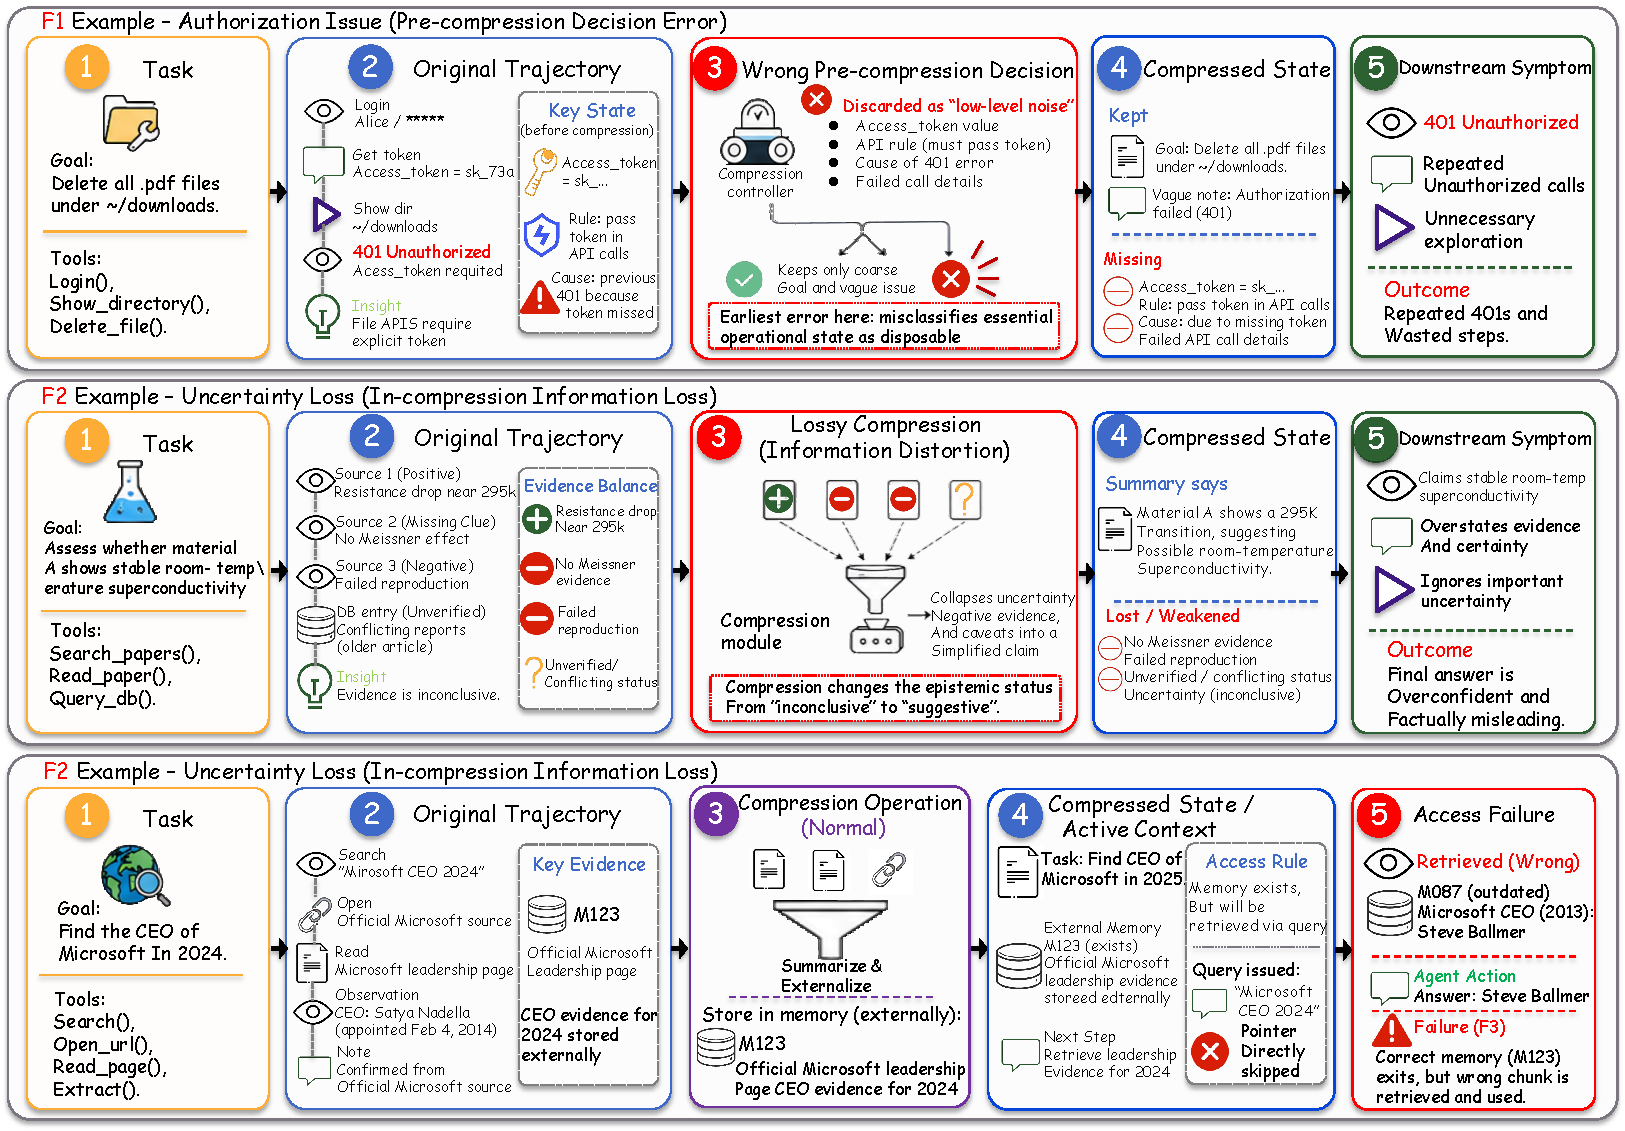
\includegraphics[width=\textwidth]{figures/cases123.pdf}
%     \caption{
%     Three illustrative cases of context compression failure modes. 
%     F1 shows a pre-compression decision error, where the compression controller misclassifies authentication state and API-call details as low-level noise before summarization. 
%     F2 shows in-compression information loss, where a compression module distorts the evidential balance by weakening uncertainty, negative evidence, and caveats. 
%     F3 shows a post-compression access failure, where the correct memory item exists after compression but is not correctly expanded or retrieved, causing the agent to use an outdated wrong chunk.
%     }
%     \label{fig:case-studies-compression-failures}
% \end{figure*}

\subsection{F1 Example -- Authorization State Dropped}
\label{app:case-f1-auth-state}

Figure~\ref{fig:case-studies-compression-failures}a illustrates an F1 failure in a file-management task. 
The agent is asked to delete all \texttt{.pdf} files under \texttt{\textasciitilde/downloads}. 
In the original trajectory, the agent logs in, obtains an \texttt{access\_token}, attempts to inspect the target directory, and observes a \texttt{401 Unauthorized} response. 
The failed API call is not merely an incidental error: it reveals an operational rule that every subsequent file-system API call must explicitly pass the access token.

The crucial state before compression therefore consists of three linked pieces of information: the concrete token value, the API rule requiring the token, and the cause of the previous \texttt{401} error. 
However, the compression controller makes a wrong pre-compression retention decision. 
It treats the token, the failed API-call details, and the token-passing rule as disposable low-level execution noise, while preserving only the coarse task objective and a vague note that authorization failed.

The resulting compressed state is insufficient for correct continuation. 
After compression, the downstream agent still knows that it should delete PDFs under the target directory, but it no longer knows how to perform authorized API calls. 
It therefore repeats unauthorized calls and wastes steps on unnecessary exploration.

This is an F1 failure because the earliest causal error occurs before the compression operation itself. 
The problem is not that the summarizer distorted selected content, nor that a saved memory could not be retrieved later. 
Rather, the controller incorrectly decided that essential operational state was not worth preserving. 
The repeated \texttt{401} errors are downstream symptoms of this pre-compression decision error.

\subsection{F2 Example -- Uncertainty Loss}
\label{app:case-f2-uncertainty-loss}

Figure~\ref{fig:case-studies-compression-failures}b illustrates an F2 failure in a research-agent task. 
The agent is asked to assess whether Material A shows stable room-temperature superconductivity. 
The original trajectory contains heterogeneous evidence: one source reports a resistance drop near 295K, another reports no Meissner evidence, a third source reports failed reproduction, and a database entry marks the claim as unverified with conflicting reports. 
The agent's intermediate conclusion is therefore cautious: the evidence is inconclusive.

Unlike the F1 case, the relevant evidence has been collected and is available to the compression module. 
The failure occurs during compression. 
When the trajectory is condensed, the compression module collapses the evidence balance into a simplified statement that Material A shows a 295K transition, suggesting possible room-temperature superconductivity. 
At the same time, the negative and uncertainty-bearing evidence is weakened or dropped: the lack of Meissner evidence, failed reproduction, unverified database status, and overall inconclusiveness no longer strongly constrain the compressed state.

This is an F2 failure because the compression process changes the epistemic status of the trajectory. 
The original evidence supports an inconclusive assessment, but the compressed state makes the claim appear more suggestive and better supported than it actually is. 
The downstream agent then overstates the evidence and produces an overconfident, factually misleading final answer.

The key distinction from F1 is that the information was not excluded by a prior retention decision. 
Instead, the evidence entered the compression step but was transformed into a less faithful representation. 
Thus, the earliest causal error lies inside the compression operation itself.

\subsection{F3 Example -- Wrong Retrieval}
\label{app:case-f3-wrong-retrieval}

Figure~\ref{fig:case-studies-compression-failures}c illustrates an F3 failure in a web-research task. 
The agent must find the CEO of Microsoft in 2024. 
In the original trajectory, it searches for ``Microsoft CEO 2024'', opens an official Microsoft source, reads the leadership page, and observes that Satya Nadella was appointed Chief Executive Officer of Microsoft on February 4, 2014. 
This correct evidence is then summarized and externalized as memory item \texttt{M123}, which stores the official Microsoft leadership evidence for the 2024 CEO.

Unlike the F2 case, the relevant information is not lost or distorted during compression. 
The compression operation successfully externalizes the correct evidence. 
However, the compressed active context does not contain the full content of \texttt{M123}; it contains the task, an external memory pointer, and an access mechanism indicating that the evidence should be retrieved when needed. 
The correct memory therefore exists, but it must re-enter the active context through a post-compression access step.

The failure occurs after compression. 
Instead of directly expanding the correct pointer \texttt{M123}, the agent issues the query ``Microsoft CEO 2024''. 
The retrieval mechanism returns a different memory item, \texttt{M087}, which is topically related but temporally mismatched: it states that Steve Ballmer was Microsoft CEO in 2013 based on an older article. 
The downstream agent integrates this wrong retrieved chunk into the active context and answers Steve Ballmer.

This is an F3 failure because the correct information has been retained, but it is not correctly accessed at the decision point. 
The earliest causal error is neither a pre-compression decision error nor an in-compression distortion. 
Rather, it is a post-compression access failure: the correct memory item \texttt{M123} exists, but the retrieval or expansion mechanism surfaces \texttt{M087} instead. 
The final answer is wrong because the agent reasons from the wrong retrieved memory, not because the correct evidence was never stored.


\section{Extended Future Directions}
\label{ap:extended_future_directions}

\paragraph{The Compression--Retrieval--Memory Boundary}
In current agent systems, compression, retrieval, and external memory are often combined, but they serve different functions and have different recoverability properties. A more principled framework is needed to determine when information should be compressed, when it should be stored externally, and when it should remain in active context.


\paragraph{Learning to Compress Recoverably}
Most existing learned policies optimize task success and token efficiency, but these objectives do not directly capture whether compressed information can be reconstructed when needed. Future work should incorporate recoverability and dependency preservation into both training objectives and evaluation.

\paragraph{Compression in Multi-Agent Systems}
When context is shared across agents, compression becomes a communication and coordination problem rather than a local memory optimization problem. This setting raises new questions about what should be summarized, what should be shared verbatim, and how compression errors propagate across agents.

\paragraph{End-to-End Training under Context Budgets}
Compression is usually treated as a separate module from planning and tool use, even though these decisions are tightly coupled in long-horizon agents. Joint optimization under explicit budget constraints may better align compression behavior with downstream task performance.

\paragraph{Domain-Specific Compression Methods}
As shown in \S~\ref{sec:5_domain_specific_analysis}, coding, web/GUI, and research agents impose different requirements on structural fidelity, recoverability, and evidence precision. This suggests that domain-tailored compression strategies will be important in addition to general-purpose methods.

\paragraph{Standardized Benchmarks and Reproducibility}
Existing work differs widely in agent backbone, task set, budget, and compressed target, which makes direct comparison difficult. Future benchmarks should report not only task success and token savings, but also information density, recoverability, error propagation, and controller overhead under controlled settings.

\paragraph{Concluding Discussion}

Agent context compression is no longer just a preprocessing convenience. For long-horizon agents, it is a state-management problem over a changing workspace, not a one-shot prompt-shortening step. This survey structures the area along three axes: targets, mechanisms, and control policies. It also introduces a failure taxonomy and an evaluation framework that goes beyond task success. The key challenge is not only stronger compression, but compression that remains recoverable, faithful, and aligned with long-term agent execution.


\newcommand{\coding}[1][1.1em]{
\includegraphics[width=#1]{icons/coding.pdf}}
\newcommand{\web}[1][1.3em]{
\includegraphics[width=#1]{icons/web.pdf}}
\newcommand{\search}[1][1.2em]{
\includegraphics[width=#1]{icons/search.pdf}}
\newcommand{\gui}[1][1.2em]{
\includegraphics[width=#1]{icons/gui.pdf}}
\newcommand{\research}[1][1.2em]{
\includegraphics[width=#1]{icons/research.pdf}}
\newcommand{\general}[1][1.2em]{
\includegraphics[width=#1]{icons/general.pdf}}

\captionsetup[longtable]{belowskip=0.5em}  % 调整这个值，正值增加距离

% Table 2 (EMNLP style, auto page-break + auto line-wrap version)
% This file is self-contained for two-column papers:
% temporarily switch to one-column so longtable can work, then switch back.

\clearpage
\onecolumn

\footnotesize
\setlength{\tabcolsep}{2pt}
\renewcommand{\arraystretch}{1.06}

% Force wrapping behavior in every cell (including long tokens / URLs-like strings).
\sloppy

% Keep total width within one-column text width to avoid overfull hboxes.
\begin{longtable}{>{\raggedright\arraybackslash\hspace{0pt}}p{0.5cm} >{\raggedright\arraybackslash\hspace{0pt}}p{2.25cm} >{\raggedright\arraybackslash\hspace{0pt}}p{2.4cm} >{\raggedright\arraybackslash\hspace{0pt}}p{2.50cm} >{\raggedright\arraybackslash\hspace{0pt}}p{2.50cm} >{\raggedright\arraybackslash\hspace{0pt}}p{2.50cm} >{\raggedright\arraybackslash\hspace{0pt}}p{1.50cm}}

\toprule[1.5pt]
\textbf{ID} & \textbf{Method} & \textbf{Author \& Year} & \textbf{When} & \textbf{What} & \textbf{How} & \textbf{Domain} \\
\hline
\endfirsthead

\multicolumn{7}{r}{\footnotesize Continued from previous page} \\
\toprule[1.5pt]
\textbf{ID} & \textbf{Method} & \textbf{Author} & \textbf{When} & \textbf{What} & \textbf{How} & \textbf{Domain} \\
\hline
\endhead

\hline
\multicolumn{7}{r}{\footnotesize Continued on next page} \\
\endfoot

\bottomrule[1.5pt]

\caption{Full Taxonomy Coordinates. Domain icons: \coding[0.85em]~Coding Agents, \web[0.85em]~Web Agents, \gui[0.85em]~GUI Interaction Agents, \search[0.85em]~Deep-Search Agents, \research[0.85em]~Research Agents, \general[0.85em]~General Agents.}
\label{tab:full_taxonomy} \\
\endlastfoot


1 & WebAgent & \citealp{gur2024realworldwebagentplanninglong} & System-Controlled & Observation & Summarization \& Abstraction & \web \gui \\
2 & PAL-UI & \citealp{liu2025paluiplanningactivelookback} & Agent-Controlled & Trajectory & Externalization \& Retrieval & \web \gui \\
3 & LCoW & \citealp{lee2025learningcontextualizewebpages} & Learned & Observation & Summarization \& Abstraction & \web \gui \\
4 & Sculptor & \citealp{li2025sculptorempoweringllmscognitive} & Agent-Controlled & Memory State & Truncation \& Masking / Abstraction & \general \\
5 & SWE-Pruner & \citealp{wang2026sweprunerselfadaptivecontextpruning} & Learned & Observation & Pruning \& Reduction & \coding \\
6 & AgentOCR & \citealp{feng2026agentocrreimaginingagenthistory} & Agent-Controlled & Trajectory & Representation-Level & \search \research \\
7 & Step-DeepResearch & \citealp{hu2025stepdeepresearchtechnicalreport} & System-Controlled & Observation & Externalization \& Retrieval & \search \research \\
8 & MCP-Bench & \citealp{wang2025mcpbenchbenchmarkingtoolusingllm} & System-Controlled & Observation & Summarization \& Abstraction & \general \\
9 & PAACE & \citealp{yuksel2025paaceplanawareautomatedagent} & Learned & Plan \& Reasoning & Pruning / Abstraction & \general \\
10 & WebWeaver & \citealp{li2025webweaverstructuringwebscaleevidence} & Agent-Controlled & Memory State & Externalization \& Retrieval & \search \research \\
11 & The Complexity Trap & \citealp{lindenbauer2025complexitytrapsimpleobservation} & System-Controlled & Observation & Truncation \& Masking & \coding \\
12 & WebClipper & \citealp{wang2026webclipperefficientevolutionweb} & Learned & Trajectory & Pruning \& Reduction & \search \research \\
13 & AOI & \citealp{bai2026aoicontextawaremultiagentoperations} & System-Controlled & Memory State & Summarization \& Abstraction & \coding \\
14 & COMPASS & \citealp{wan2025compassenhancingagentlonghorizon} & External Controller & Plan \& Reasoning & Summarization \& Abstraction & \search \research \\
15 & ACC & \citealp{bousetouane2026aiagentsneedmemory} & External Controller & Memory State & Summarization \& Abstraction & \general \\
16 & BACM & \citealp{xiao2025improving} & Agent-Controlled & Trajectory & Summarization \& Abstraction & \search \research \\
17 & Q-KVComm & \citealp{kriuk2025qkvcommefficientmultiagentcommunication} & System-Controlled & Representation-Level & Representation-Level & \general \\
18 & Visual MAD & \citealp{wu2026crossmodalmemorycompressionefficient} & System-Controlled & Trajectory & Representation-Level & \general \\
19 & SCMA & \citealp{chen2026selfcompressionchainofthoughtmultiagentreinforcement} & Learned & Plan \& Reasoning & Pruning \& Reduction & \general \\
20 & CSIM & \citealp{liu2025csim} & Learned & Plan \& Reasoning & Summarization \& Abstraction & \search \research \\
21 & ACON & \citealp{kang2025aconoptimizingcontextcompression} & Learned & Trajectory / Observation & Summarization \& Abstraction & \coding \\
22 & SAC & \citealp{liu2026autoencodingfreecontextcompressionllms} & System-Controlled & Representation-Level & Representation-Level & \general \\
23 & PoC & \citealp{zhao2026pocperformanceorientedcontextcompression} & External Controller & Trajectory / Observation & Pruning / Abstraction & \general \\
24 & SWE-AGILE & \citealp{lian2026sweagilesoftwareagentframework} & Learned & Plan \& Reasoning & Truncation / Abstraction & \coding \\
25 & LoCoEval Framework & \citealp{liu2026scalablebenchmarkrepositoryorientedlonghorizon} & System-Controlled & Memory State & Externalization \& Retrieval & \coding \\
26 & LongSeeker & \citealp{lu2026longseekerelasticcontextorchestration} & Agent-Controlled & Trajectory & Pruning / Abstraction / Retrieval & \search \research \\
27 & Context-Folding & \citealp{sun2025scalinglonghorizonllmagent} & Agent-Controlled & Trajectory & Summarization \& Abstraction & \general \\
28 & ContextWeaver & \citealp{wu2026contextweaverselectivedependencystructuredmemory} & External Controller & Memory State & Pruning \& Reduction & \general \\
29 & HIAGENT & \citealp{hu-etal-2025-hiagent} & Agent-Controlled & Plan \& Reasoning & Summarization \& Abstraction & \general \\
30 & ProMem & \citealp{yang2026staticsummarizationproactivememory} & Agent-Controlled & Memory State & Summarization \& Abstraction & \general \\
31 & OCR-Memory & \citealp{li2026ocrmemoryopticalcontextretrieval} & External Controller & Memory State & Externalization \& Retrieval & \web \gui \\
32 & AgentDiet & \citealp{xiao2025improving} & System-Controlled & Trajectory & Pruning \& Reduction & \coding \\
33 & AgentProg & \citealp{tian2026agentprogempoweringlonghorizongui} & System-Controlled & Memory State & Pruning \& Reduction & \web \gui \\
34 & GCC & \citealp{wu2026gitcontextcontrollermanage} & Agent-Controlled & Memory State & Externalization \& Retrieval & \general \\
35 & TACO & \citealp{ren2026selfevolvingframeworkefficientterminal} & Learned & Observation & Pruning \& Reduction & \coding \\
36 & CodeOCR & \citealp{shi2026codeocr} & System-Controlled & Observation & Representation-Level & \coding \\
37 & AttentionRAG & \citealp{fang2025attentionrag} & System-Controlled & Observation & Pruning \& Reduction & \general \\
38 & LongCodeZip & \citealp{shi2025longcodezip} & System-Controlled & Observation & Pruning \& Reduction & \coding \\
39 & ReSum & \citealp{wu2026resumunlockinglonghorizonsearch} & System-Controlled & Trajectory & Summarization \& Abstraction & \search \research \\
40 & Focus & \citealp{verma2026activecontextcompressionautonomous} & Agent-Controlled & Trajectory & Pruning \& Reduction & \coding \\
41 & AgentFold & \citealp{ye2025agentfoldlonghorizonwebagents} & Agent-Controlled & Trajectory & Summarization \& Abstraction & \search \research \\
42 & CAT & \citealp{liu2025contexttoolcontextmanagement} & Agent-Controlled & Trajectory & Summarization \& Abstraction & \coding \\
43 & MEM1 & \citealp{zhou2025mem1learningsynergizememory} & Learned & Memory State & Summarization \& Abstraction & \general \\
44 & ContextEvolve & \citealp{su2026contextevolvemultiagentcontextcompression} & External Controller & Memory State & Summarization \& Abstraction & \coding \\

\end{longtable}

\clearpage
\twocolumn
% Open-source methods table (two-column wide)
\begin{table*}[htbp]
\centering
\footnotesize
\setlength{\tabcolsep}{5pt}
\renewcommand{\arraystretch}{1.12}
\begin{tabular}{p{0.30\textwidth}p{0.54\textwidth}p{0.08\textwidth}}
\toprule[1.5pt]
\textbf{Method} & \textbf{Open-source link} & \textbf{Year} \\
\midrule
SWE-Pruner~\citep{wang2026sweprunerselfadaptivecontextpruning} & \url{https://github.com/Ayanami1314/swe-pruner} & 2026 \\
Step-DeepResearch~\citep{hu2025stepdeepresearchtechnicalreport} & \url{https://github.com/stepfun-ai/StepDeepResearch} & 2025 \\
MCP-Bench~\citep{wang2025mcpbenchbenchmarkingtoolusingllm} & \url{https://github.com/Accenture/mcp-bench} & 2025 \\
WebWeaver~\citep{li2025webweaverstructuringwebscaleevidence} & \url{https://github.com/Alibaba-NLP/DeepResearch} & 2025 \\
The Complexity Trap~\citep{lindenbauer2025complexitytrapsimpleobservation} & \url{https://github.com/JetBrains-Research/the-complexity-trap} & 2025 \\
WebClipper~\citep{wang2026webclipperefficientevolutionweb} & \url{https://github.com/AQ-MedAI/AntAFu-DeepResearch} & 2026 \\
ACON~\citep{kang2025aconoptimizingcontextcompression} & \url{https://github.com/microsoft/acon} & 2025 \\
SAC~\citep{liu2026autoencodingfreecontextcompressionllms} & \url{https://github.com/lx-Meteors/SAC} & 2026 \\
SWE-AGILE~\citep{lian2026sweagilesoftwareagentframework} & \url{https://github.com/KDEGroup/SWE-AGILE} & 2026 \\
HIAGENT~\citep{hu-etal-2025-hiagent} & \url{https://github.com/HiAgent2024/HiAgent} & 2025 \\
AgentProg~\citep{tian2026agentprogempoweringlonghorizongui} & \url{https://github.com/MobileLLM/AgentProg} & 2026 \\
GCC~\citep{wu2026gitcontextcontrollermanage} & \url{https://github.com/theworldofagents/GCC} & 2026 \\
TACO~\citep{ren2026selfevolvingframeworkefficientterminal} & \url{https://github.com/multimodal-art-projection/TACO} & 2026 \\
CodeOCR~\citep{shi2026codeocr} & \url{https://github.com/YerbaPage/CodeOCR} & 2026 \\
LongCodeZip~\citep{shi2025longcodezip} & \url{https://github.com/YerbaPage/LongCodeZip} & 2025 \\
ReSum~\citep{wu2026resumunlockinglonghorizonsearch} & \url{https://github.com/Alibaba-NLP/DeepResearch} & 2026 \\
AgentFold~\citep{ye2025agentfoldlonghorizonwebagents} & \url{https://github.com/Alibaba-NLP/DeepResearch} & 2025 \\
MEM1~\citep{zhou2025mem1learningsynergizememory} & \url{https://github.com/MIT-MI/MEM1} & 2025 \\
ContextEvolve~\citep{su2026contextevolvemultiagentcontextcompression} & \url{https://anonymous.4open.science/r/ContextEvolve-ACC} & 2026 \\
\bottomrule[1.5pt]
\end{tabular}
\caption{Open-source methods included in this survey.}
\label{tab:opensource_methods}
\end{table*}

\definecolor{lightblue}{HTML}{ADD8E6}
\definecolor{starlight}{HTML}{F9F7ED}
\definecolor{lightgray}{HTML}{EEEEEE}

\begin{figure*}[t]
\centering
\resizebox{1.0\textwidth}{!}{
\begin{tikzpicture}[scale=1.0]
\genealogytree[
level 2/.style={level size=11.5cm,node box={colback=lightgray}},
level 1/.style={level size=2.3cm,node box={colback=starlight},further distance=1mm},
level 0/.style={level size=2.5cm,node box={colback=lightblue,rotate=90}},
timeflow=left,
processing=tcolorbox,
node size from=5mm to 4cm,
box={size=small,halign=center,valign=center,fontupper=\footnotesize\textrm{}},
edges={foreground=black!25,background=black!5},
class1/.style={box={colback=lightgray}},
class2/.style={box={colback=starlight}},
class3/.style={box={colback=lightblue}},
level distance=5mm,
]
{
    parent{
        g[class3]{\scriptsize Domain}
            parent{
                g[class2]{\scriptsize General}
                p[class1,id=general]{\tiny Sculptor~\cite{li2025sculptorempoweringllmscognitive}, MCP-Bench~\cite{wang2025mcpbenchbenchmarkingtoolusingllm}, PAACE~\cite{yuksel2025paaceplanawareautomatedagent}, Q-KVComm~\cite{kriuk2025qkvcommefficientmultiagentcommunication}, SAC~\cite{liu2026autoencodingfreecontextcompressionllms}, SCMA~\cite{chen2026selfcompressionchainofthoughtmultiagentreinforcement}, CSIM~\cite{liu2025csim}, ACC~\cite{bousetouane2026aiagentsneedmemory}, PoC~\cite{zhao2026pocperformanceorientedcontextcompression}, Context-Folding~\cite{sun2025scalinglonghorizonllmagent}, HIAGENT~\cite{hu-etal-2025-hiagent}, ProMem~\cite{yang2026staticsummarizationproactivememory}, ContextEvolve~\cite{su2026contextevolvemultiagentcontextcompression}, MEM1~\cite{zhou2025mem1learningsynergizememory}}
                }
            parent{
                g[class2]{\scriptsize Coding}
                p[class1,id=coding]{\tiny SWE-Pruner~\cite{wang2026sweprunerselfadaptivecontextpruning}, The Complexity Trap~\cite{lindenbauer2025complexitytrapsimpleobservation}, ACON~\cite{kang2025aconoptimizingcontextcompression}, SWE-AGILE~\cite{lian2026sweagilesoftwareagentframework}, AgentDiet~\cite{xiao2025improving}, AgentProg~\cite{tian2026agentprogempoweringlonghorizongui}, CodeOCR~\cite{shi2026codeocr}, LongCodeZip~\cite{shi2025longcodezip}, Focus~\cite{verma2026activecontextcompressionautonomous}, CAT~\cite{liu2025contexttoolcontextmanagement}, TACO~\cite{ren2026selfevolvingframeworkefficientterminal}}
                }
            parent{
                g[class2]{\scriptsize Web \& GUI}
                p[class1,id=webgui]{\tiny WebAgent~\cite{gur2024realworldwebagentplanninglong}, PAL-UI~\cite{liu2025paluiplanningactivelookback}, LCoW~\cite{lee2025learningcontextualizewebpages}, WebWeaver~\cite{li2025webweaverstructuringwebscaleevidence}, WebClipper~\cite{wang2026webclipperefficientevolutionweb}, OCR-Memory~\cite{li2026ocrmemoryopticalcontextretrieval}, Sculptor~\cite{li2025sculptorempoweringllmscognitive}, AOI~\cite{bai2026aoicontextawaremultiagentoperations}, Visual MAD~\cite{wu2026crossmodalmemorycompressionefficient}, AgentProg~\cite{tian2026agentprogempoweringlonghorizongui}}
                }
            parent{
                g[class2]{\scriptsize Research \& Deep-Search}
                p[class1,id=research]{\tiny Step-DeepResearch~\cite{hu2025stepdeepresearchtechnicalreport}, AgentOCR~\cite{feng2026agentocrreimaginingagenthistory}, WebWeaver~\cite{li2025webweaverstructuringwebscaleevidence}, COMPASS~\cite{wan2025compassenhancingagentlonghorizon}, BACM~\cite{xiao2025improving}, LongSeeker~\cite{lu2026longseekerelasticcontextorchestration}, ReSum~\cite{wu2026resumunlockinglonghorizonsearch}, AgentFold~\cite{ye2025agentfoldlonghorizonwebagents}}
                }
        }
}
\end{tikzpicture}}
\caption{A taxonomy of context management methods from the perspective of domain.}
\label{fig:domain_taxonomy}
\end{figure*}
% Datasets / benchmarks table for context management survey
% This file is self-contained: it includes the table, introductory text,
% and notes that can be inserted directly into the main paper.

\clearpage
\onecolumn

\footnotesize
\setlength{\tabcolsep}{4.2pt}
\renewcommand{\arraystretch}{1.12}
\sloppy

\begin{longtable}{>{\raggedright\arraybackslash\hspace{0pt}}p{5.65cm} >{\raggedright\arraybackslash\hspace{0pt}}p{2.55cm} >{\raggedright\arraybackslash\hspace{0pt}}p{7.00cm}}
\toprule[1.5pt]
\textbf{Benchmark} & \textbf{Source \& year} & \textbf{Open Source} \\
\midrule
\endfirsthead

\toprule[1.5pt]
\textbf{Benchmark} & \textbf{Source \& year} & \textbf{Open Source} \\
\midrule
\endhead

\midrule
\multicolumn{3}{r}{\footnotesize Continued on next page} \\
\endfoot

\bottomrule[1.5pt]
\caption{Representative datasets and benchmarks for agent context management.}
\label{tab:datasets_benchmarks}
\endlastfoot

SWE-bench Verified~\citep{jimenez2024swebench} & ICLR 2024 & \url{https://huggingface.co/datasets/SWE-bench/SWE-bench_Verified} \\
GAIA~\citep{mialon2023gaia} & arXiv 2023 & \url{https://huggingface.co/datasets/gaia-benchmark/GAIA} \\
BrowseComp~\citep{wei2025browsecomp} & arXiv 2025 & \url{https://github.com/openai/simple-evals} \\
BrowseComp-Plus~\citep{chen2025browsecompplus} & ACL 2026 & \url{https://huggingface.co/datasets/Tevatron/browsecomp-plus} \\
BrowseComp-ZH~\citep{zhou2025browsecompzh} & arXiv 2025 & \url{https://huggingface.co/datasets/PALIN2018/BrowseComp-ZH} \\
Mind2Web~\citep{deng2023mind2web} & NeurIPS 2023 & \url{https://huggingface.co/datasets/osunlp/Mind2Web} \\
Multimodal-Mind2Web~\citep{zheng2024seeact} & ICML 2024 & \url{https://huggingface.co/datasets/osunlp/Multimodal-Mind2Web} \\
HLE~\citep{phan2025humanitys} & arXiv 2025 & \url{https://huggingface.co/datasets/cais/hle} \\
AppWorld~\citep{trivedi2024appworld} & ACL 2024 & \url{https://github.com/StonyBrookNLP/appworld} \\
OfficeBench~\citep{wang2024officebench} & arXiv 2024 & \url{https://github.com/zlwang-cs/OfficeBench} \\
HotpotQA~\citep{yang2018hotpotqa} & EMNLP 2018 & \url{https://hotpotqa.github.io/} \\
Natural Questions~\citep{kwiatkowski2019natural} & TACL 2019 & \url{https://github.com/google-research-datasets/natural-questions} \\
TriviaQA~\citep{joshi2017triviaqa} & ACL 2017 & \url{http://nlp.cs.washington.edu/triviaqa/} \\
GSM8K~\citep{cobbe2021training} & arXiv 2021 & \url{https://github.com/openai/grade-school-math} \\
MATH / MATH-500~\citep{hendrycksmath2021} & NeurIPS 2021 & \url{https://github.com/hendrycks/math} \\
SWE-bench Lite~\citep{jimenez2024swebench} & ICLR 2024 & \url{https://huggingface.co/datasets/princeton-nlp/SWE-bench_Lite} \\
ALFWorld~\citep{shridhar2021alfworld} & ICLR 2021 & \url{https://github.com/alfworld/alfworld} \\
WebShop~\citep{yao2022webshop} & NeurIPS 2022 & \url{https://github.com/princeton-nlp/webshop} \\
AndroidWorld / AW-Extend~\citep{rawles2024androidworld} & ICLR 2025 & \url{https://github.com/google-research/android_world} \\
DeepResearch Bench~\citep{du2025deepresearch} & arXiv 2025 & \url{https://github.com/Ayanami0730/deep_research_bench} \\
TerminalBench (TB 1.0 / 2.0)~\citep{merrill2026terminalbench} & arXiv 2026 & \url{https://github.com/harbor-framework/terminal-bench} \\
MRQA~\citep{fisch-etal-2019-mrqa} & EMNLP WS 2019 & \url{https://huggingface.co/datasets/mrqa} \\
CodeXGLUE~\citep{lu2021codexglue} & NeurIPS / FSE 2021 & \url{https://github.com/microsoft/CodeXGLUE} \\
AIOpsLab~\citep{chen2025aiopslab} & MLSys 2025 & \url{https://microsoft.github.io/AIOpsLab/} \\
Loghub~\citep{zhu2023loghub} & ISSRE 2023 & \url{https://github.com/logpai/loghub} \\
LongBench~\citep{bai2024longbench} & MLSys 2024 & \url{https://huggingface.co/datasets/THUDM/LongBench} \\
LongBench V2~\citep{bai2025longbenchv2} & ACL 2025 & \url{https://longbench2.github.io} \\
BABILong~\citep{NEURIPS2024_babilong} & NeurIPS 2024 & \url{https://github.com/booydar/babilong} \\
ADRS Benchmark~\citep{cheng2025barbarians} & arXiv 2025 & \url{https://github.com/UCB-ADRS/ADRS} \\
WorkArena~\citep{drouin2024workarena} & ICML 2024 & \url{https://github.com/ServiceNow/WorkArena} \\
MiniWoB~\citep{shi2017world} & ICML 2017 & \url{https://miniwob.farama.org/} \\
MiniWoB++~\citep{liu2018reinforcement} & ICLR 2018 & \url{https://miniwob.farama.org/} \\
NeedleBench~\citep{li2024needlebench} & arXiv 2024 & \url{https://github.com/open-compass/opencompass} \\
NIAH~\citep{liu2023lost} & arXiv 2023 & \url{https://github.com/open-compass/opencompass} \\
HaluMem~\citep{chen2025halumem} & arXiv 2025 & \url{https://huggingface.co/datasets/IAAR-Shanghai/HaluMem} \\
LongMemEval~\citep{wu2025longmemeval} & ICLR 2025 & \url{https://huggingface.co/datasets/xiaowu0162/longmemeval-cleaned} \\
LoCoEval Framework~\citep{liu2026scalable} & arXiv 2026 & - \\
DevEval~\citep{li2024deveval} & ACL Findings 2024 & \url{https://github.com/seketeam/DevEval} \\
WideSearch~\citep{wong2025widesearch} & ICLR 2026 & \url{https://huggingface.co/datasets/ByteDance-Seed/WideSearch} \\
CompileBench / CRUST-Bench~\citep{khatry2025crustbench} & COLM 2025 & \url{https://github.com/QuesmaOrg/CompileBench} \\
GovReport~\citep{huang-etal-2021-efficient} & NAACL 2021 & \url{https://gov-report-data.github.io/} \\
SummScreenFD~\citep{chen-etal-2022-summscreen} & ACL 2022 & \url{https://gov-report-data.github.io/} \\
\end{longtable}

\clearpage
\twocolumn



% \noindent
% \colorbox{violet!8}{
% \begin{minipage}{0.48\textwidth}
% \small{
% \color{violet}{\textbf{\raisebox{-0.15em}{
\includegraphics[height=1em]{icons/idea.pdf}}~Summary \& Ideas}}}
% \begin{itemize}[itemsep=-1pt, topsep=2pt, leftmargin=6pt, labelsep=3pt]
% \item *************************.  
% \item *************************.
% \item *************************. 
% \end{itemize}
% \end{minipage}
% }

\end{document}
